\documentclass[letterpaper,twocolumn,10pt]{article}
\usepackage{usenix,epsfig,endnotes}
%\hyphenation{op-tical net-works semi-conduc-tor}

\usepackage{multirow}
\usepackage{amsmath,amssymb}
\usepackage{theorem}
\usepackage{tabularx}
%\usepackage[dvipdfmx]{graphicx}
%\usepackage{bmpsize}
\usepackage{subfigure}
%\usepackage[ruled,linesnumbered,vlined]{algorithm2e}
\usepackage{hyperref}
\usepackage{url}
%\usepackage{algorithm2e}
\usepackage{comment}
%\usepackage{algorithmic}
\usepackage{multicol}
\usepackage{multirow}
\usepackage{tabularx}
\usepackage{amsmath,amssymb}
\usepackage{theorem}
\usepackage{multibib}
\usepackage{color}
\usepackage{algorithm,algpseudocode}
\usepackage{longtable}
\usepackage{rotating}
\usepackage{hhline}
\usepackage{supertabular}
\usepackage{booktabs}
\usepackage{hyperref}
\usepackage{float}
\usepackage[switch]{lineno}



\theoremstyle{plain} \newtheorem{theorem}{Theorem}
\theoremstyle{plain} \newtheorem{definition}{Definition}
\theoremstyle{plain} \newtheorem{lemma}{Lemma}
\theoremstyle{plain} \newtheorem{remark}{Remark}
\theoremstyle{plain} \newtheorem{proof}{Proof}

\renewcommand{\multirowsetup}{\centering}
%\newcommand{\algo}[]{}
\makeatletter
%\def\@seccntformatinl#1{\csname the#1dis\endcsname\hskip 1em\relax}
%\makeatother


\begin{document}
\date{}

\title{\Large \bf A High Efficient Two-Hierarchies Tensor-Embedding-Aware App Clone Detection System}

\author{
{\rm Your N.\ Here}\\
Your Institution
\and
{\rm Second Name}\\
Second Institution
% copy the following lines to add more authors
% \and
% {\rm Name}\\
%Name Institution
} 

\maketitle

% Use the following at camera-ready time to suppress page numbers.
% Comment it out when you first submit the paper for review.
\thispagestyle{empty}


\subsection*{Abstract}
App homology analysis tasks on binary codes are expected to be scalable and effective. However, most works have a complex training process or are slow and less capable of catching new increasing apps. We use two hierarchies' embedding model to obtain concise and accurate feature vector, which represents binary codes of the app. In our research, firstly, we implement a novel first-hierarchy embedding prototype for the control flow graph (CFG) of app's binary codes called 5UD-CFG that preserves the global CFG structure. Secondly, we propose the compression, clustering and update algorithms according to the proposed second-hierarchy tensor embedding model to obtain a more concise and accurate feature numeric vector called 3TU-CFG for app's binary codes. This model abandons the complex learning process of existing effective works that are based on the neural network or other learning algorithms. Thirdly, Empirical experiments prove that the effectiveness of two hierarchies CFG embedding on app homology analysis detection. 3TU-CFG run $4\times$ to $76000\times$ faster than the existing works' preprocessing and at least reduce the half of search time. At the same time, the homoloy detection accuracy approximates $99\%$.   

%\IEEEdisplaynotcompsoctitleabstractindextext

%\IEEEpeerreviewmaketitle
\section{Introduction}
The study of the app homology has recently emerged as a major catalyst for collectively understanding the behavior of complex app in the mobile.  Thousands, and millions of apps have been used around the world from various app markets, such as PP assistant, Android, Google Play, SnapPea and tens of smaller third-party markets. With the rapidly increasing use of apps, code clone, malware code injection bring several serious finance threats. With this prosperity, app homology can be used in the malware detection, plagiarism detection, etc. More than $85\%$ of Android malware rely on app clone to spread to a large number of genuine users \cite{ZhouJ12}, for example, crack paid apps to bypass payment function, modify the advertisement libraries, or even insert various malicious functions, which lead to a serious security problem for the mobile application. Specifically, app developers and security researchers urgently need to find an effective app homology method to satisfy the requirement of fast increasing apps. 
%At the same time, app homology analysis needs to solve the challenge that quickly detect similar functions directly in binaries across multiple platform. 

%As a result, the need for third-party evaluator to accurately and quickly identify benign or malware in mobile app is increasing dramatically.

However, discovering the similar app or derivative app is like distinguishing beans from a mount of jumble beads, even when we are dealing with the known app. To address this critical problem, primitive app researchers statically scans an app for known codes and operations for suspicious activities \cite{DTeuflFFHKO16}. The problem here is that the static approach does not work on new threats. Recent researchers have been actively developing techniques to automatically analyze and detect app homology in the mobile markets. There are several studies that propose the app clone technology and scalable app classification. Detection based on string \cite{Baker95}, detection based on token\cite{IwamotoON12}\cite{YuanG12}, detection based on hash \cite{ChenGZGCZ17}\cite{ZhangLZRS16}, detection based on the program dependence graph \cite{YuLYLYY16} \cite{HamidZ14} and detection based on abstract syntax tree \cite{FuXYY17} \cite{HovemeyerHPS16} \cite{KikuchiGWN15} have shown their scalability to handle thousands and millions of codes. However, some approaches generate too many false negative at handling the classification of malware with imperceptible change, such as sting-based detection, token-based detection. Some approaches are not scalable that can not handle billions of opcodes in multiple app market, such as the program dependence graph. The dynamic method can be circumvented by an app capable of fingerprinting the testing environment \cite{Spreitzenbarth13}, but the dynamic analysis can be heavyweight, which makes it hard to explore all execution paths of an app. 

%The study of data dimensionality reduction has been reported in the literature. Previous approaches include Principal Component Analysis (PCA) \cite{HanWZY18}, Incremental Singular Value Decomposition (SVD) \cite{DGorrell06} \cite{DChenC14} etc. 


There has been several specific challenges:
\begin{enumerate}
  \item There has been an primitive challenge on designing a feasible model to accurately represent scalable apps at the binary codes level. The binary codes of app are very complicated source data. They appear on different markets, and most apps' binary codes are confused. We need extract considerable features to denote binary codes. 
  \item How handle the millions and billions features of app binary codes in multiple markets to accurately analysis the app homology? There is an challenging that we need to accurately find homologous apps in the mass quantity of features of apps. 
  \item There has been facing an challenge to update the feature data for the rapidly increasing apps. Since the update of app feature data needs to relearn all apps' feature including preceding app features in the existing works. However, most existing update approaches are expensive works, and they cost too much additional time and space. We should design a update system that can incrementally and timely update the app feature data. 
\end{enumerate}

%The learning algorithm is widely used in dealing with the classification of big data. 

%Our goal is to address these challenges by proposing a suitable embedding system to transform the binary code of app to a low-dimensional feature vector. Since apps' binary codes are complex, we need to extract more concise and specific storable features represented the apps' binary codes to be easier for the app homology analysis. First, We know that the main content of a app is its smali functions. The control flow graph of the function can greatly preserve the opcode structure. We need to design a embedding approach to preserve both the opcode structure and numeric characteristics of original binary code of the app based on the control flow graph. Second, the embedding features that are extracted from the CFG of app's binary codes are scalable, we need to make the feature dimensionality reduced and compressed. The tensor computations have a great effect on data reduction. We need to propose a tensor embedding model and a compress approach to get more concise and accurate app 's feature data. Third, based on the proposed tensor embedding model, it is easier to propose a incremental update system of the app feature data. Moreover, we also need to prove the monotonicity and validity of the embedding feature theoretically and practically.

Our goal is to address these challenges by proposing a suitable embedding system to transform binary codes of the app to a low-dimensional feature vector.  First, Since apps' binary codes are complex, CFG of the function can greatly preserve the opcode structure. We need to design a embedding approach to preserve both the opcode structure and numeric characteristics of original binary code of the app based on CFG. Second, the embedding features that are extracted from the CFG of app's binary codes are scalable, and tensor computations have a great effect on data reduction. We need to make the feature dimensionality reduced and compressed. Third, based on tensor computations, it is easier to propose an incremental update system of the app features. Moreover, we also need to prove the monotonicity and the validity of embedding features theoretically and practically.
%the 5UD-CFG line embedding and 3TU-CFG tensor embedding make the app homology more scalable than current existing works.based on the extracted control flow graph with the vertex features from the app's binary codes, the two hierarchies model .  Third, the monotonicity of 5UD-CFG line embedding and the injective reversibility of 3TU-CFG tensor model are proved to make sure it more accurate than other works. The 3TU-CFG tensor model also makes the update easy for the search database of the app homology analysis. Evolution shows that finding a unknown function less than $4.6 \times 10^{(-9)}$ seconds in a thousand apps and $0.1$ seconds in $10^8$ apps.

In this paper, our interdisciplinary study focuses on leveraging two hierarchies embedding model to obtain the feature numeric vector based on the CFG of app's binary codes to handle the app homology analysis. The two hierarchies embedding model shows a more effective and accurate app homology strategy than current other works. The main contributions of our work are summarized as follows:
\begin{enumerate}
  \item We develop the first-hierarchy line embedding model for the extracting CFG that each vertex has five eigenvalues by decompiling the app, which is called as 5UD-CFG. Moreover, we can theoretically prove that first-hierarchy embedding feature 5UD-CFG can uniquely represent a CFG.
  \item We design the second-hierarchy 3TU-CFG tensor embedding model based on the extracting first-hierarchy embedding feature 5UD-CFG. Then we propose an special tensor-SVD factorization algorithm to decompose tensor model, which compress 5UD-CFG as 3TU-CFG. This is second-hierarchy embedding process that compresses and clusters the first-hierarchy embedding feature matrixes to greatly accelerate the efficiency of the match and the classification. 
  \item We propose an incremental tensor decomposition algorithm to match the compressing and clustering learning process of tenor embedding model. Compared with the existing work for the update process of the app homology analysis data, the efficiency is greatly improved $2\times$ to $18000\times$.
  \item Our evaluation shows that two hierarchies embedding process obtained feature vector can accelerate the preparation process $4\times$ to $76000\times$ faster than prior works, i.e., Gemini, Genius, Centroid. At the same time, the search and detection time run at least 1 to 2 orders of magnitude faster than prior time even though the prior search time is very minor. Evolution also shows that finding a unknown function less than $4.6 \times 10^{(-9)}$ seconds in a thousand apps and $0.1$ seconds in $10^8$ apps.
\end{enumerate}

%The remainder of the paper is structured as follows. Background of the app clone are given in Section 2. In Section 3, we introduce the  problem definition that we need to solve. In Section 4, we show the overview solution for proposed two-hierarchies embedding model. In Section 5, we propose the first-hierarchy line embedding model,  and prove the monotonicity of the proposed first-hierarchy embedding feature 5UD-CFG. In Section 6, we propose the second-hierarchy tensor embedding model based on the first-hierarchy embedding feature 5UD-CFG. Moreover, we give a learning algorithm to compress and clustering the first-class embedding feature unitary matrix to obtain a more concise embedding feature 3TU-CFG, which can be effective to handle the app homology match and detection. Section 7 illustrates the experiments to verify the efficiency and accuracy of two hierarchies embedding process. We conclude with remarks on future work in Section 8.
                                                                                                                                             

%\section{Feature Extraction }
In this section, we introduce the detailed approaches how we uniquely represent the Android apps. The CFG(Control Flow Graph) is the common feature used in bug search. Moreover, different from other attributes on the basic blocks, such as I/O pairs and statics features \cite{23}\cite{45(SGbBSfFI)}, are more accuracy matching. Following  the idea of the original CFG extraction, this paper utilizes the control flow graph with different basic-block level attributes about five features based, it called as the 5UD-CFG. We also prove the monotonicity of the feature of the 5UD-CFG. A feature of 5UD-CFG represents a CFG.

\subsection{Disassembly of Android Application and CFG extraction}
In our system, the preprocessing of an application consists of disassembling the application and extracting opcode sequences. A code file is a dex file that can be transformed into smali files, where each smali file represents a single class and contains the methods of such a class. Each method contains instructions and each instruction consists of a single opcode and multiple operands.  

After preparation, including downloading all the apps from multiple markets or malware database and extracting methods from the apps, we encode a projection form of CFG to get the unique feature of the function of an apk.

CFG is the control flow graph of a method. Each node in a CFG corresponds to a basic block in the method. A basic block is a straight-line piece of code with one entry point and one exit point. Jump targets start a block, and jump end a block. Directed edges are used to represent jumps in the control flow.

\subsection{5UD-CFG}
In this paper, we extract the unique property of CFG by a number list, which is proved monotonically represent its corresponding CFG. Android apps are written in JAVA, which is a kind of structured programming. Sequence, branch and circulation are three basic structures to encode a CFG to 5UD-CFG.

\textbf{Definition 1.} (5UD-CFG) The control flow graph with five unique feature, or 5UD-CFG in short, is a directed graph $G=<V,E>$, where $V$ is a set of basic block in a function;$E \subseteq V \times V$ is a set of edges representing the connections between these basic blocks. Each node in $V$ has a unique coordinate. The coordinate of a node is a vector $<n, s, i, o, l>$. $n$ is the sequence number of a node in the CFG, $s$ is the number of opcodes of a basic block, the $i$ is the number of input edges of the node (the basic block), $o$ is the number of outgoing edges of the node. $l$ is the number of the loop of a node.

Fig. 1 shows a real CFG of a function in a class. A node represents a basic block, and a edge represents a call link between two basic block. A basic block is a set of opcodes. The outgoing edges of a node $A$ represents the basic block $A$ is called by other basic block. The input edges of a node $A$ represents the basic block $A$ calls other basic blocks. 

\begin{figure}[hbt]
  \center{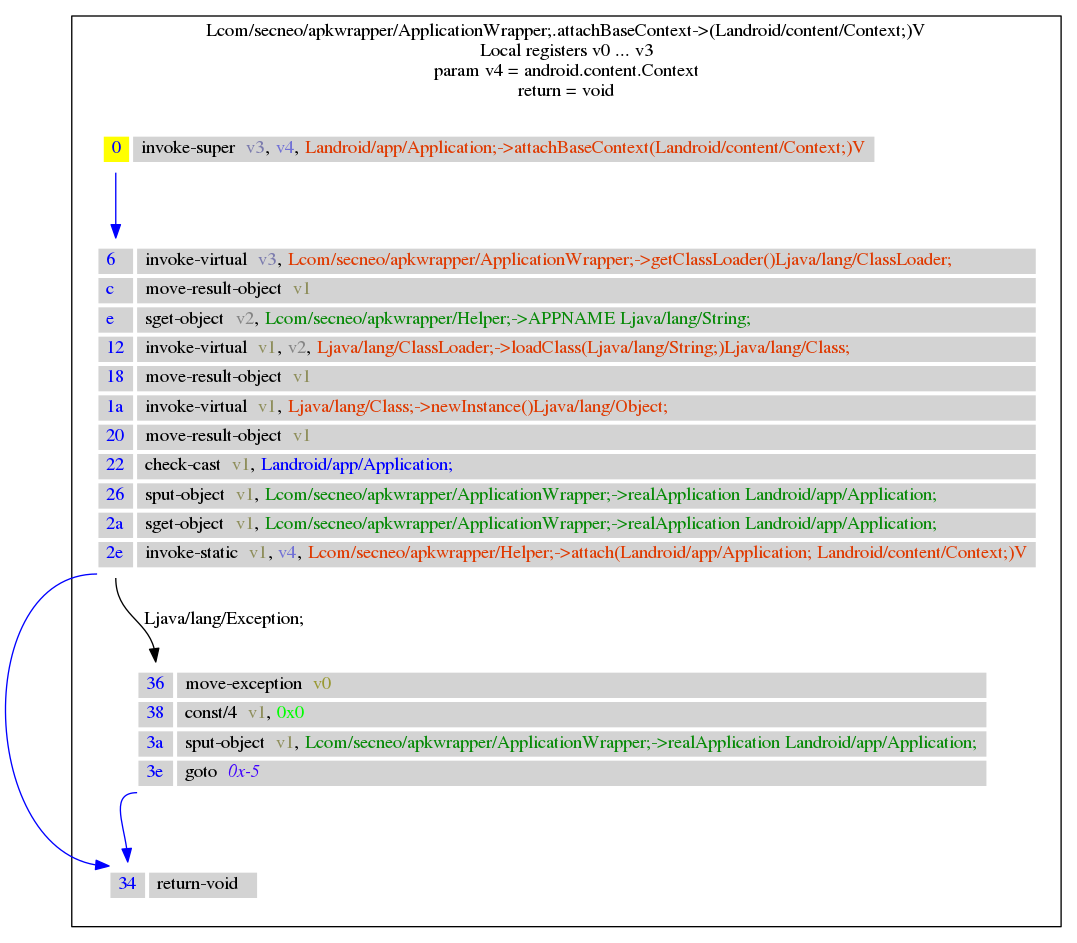
\includegraphics[width=8cm] {cfgexample.png}}
  \caption{\label{1} My figure.  An example of a method cfg in a real apk}
\end{figure}

There is a unique mapping between a CFG and a 5UD-CFG. The same node in a CFG has the same sequence number, which is decided by the order in which it executes. The entry node is with the number 1. The sequence number list of all nodes shows the result of the breadth first search in the CFG. For example, as shown in the Fig.1 and the Fig. 2, it is the CFG and the 5UD-CFG of a real method in a apk. Node $A$ in the CFG is the starting node with the sequence number 1. The sequence number of $B$ is 2, and so on $C$ is 3, $D$ is 4, and $E$ is 5. The loop of a node shows there is a directed circle from the node back to the node. The number of the loop of the $A$ is 0, $B$ is 1, $C$ is 1, $D$ is 0, and $E$ is 0. Other features are shown in the Fig. 2(b).

A 5UD-CFG can be viewed as a set of nodes connected by edges. We need to define the node weight of each node (basic block). The node weight of each node is used to combine all node to represent the CFG. We define the feature of a 5UD-CFG based on the 3D-CFG \cite{chenkai}.

\textbf{Definition 2.} A feature of a 5UD-CFG is a vector $<f_n, f_s, f_i, f_o, f_l>. f_n=\frac{\sum_{e(j,k)\in 5UD-CFG}(\omega_jn_j+\omega_kn_k)}{\omega}, \\ f_s=\frac{\sum_{e(j,k)\in 5UD-CFG}(\omega_js_j+\omega_ks_k)}{\omega}, \\ f_i=\frac{\sum_{e(j,k)\in 5UD-CFG}(\omega_ji_j+\omega_ki_k)}{\omega},\\ f_o=\frac{\sum_{e(j,k)\in 5UD-CFG}(\omega_jo_j+\omega_ko_k)}{\omega}, \\f_l=\frac{\sum_{e(j,k)\in 5UD-CFG}(\omega_jl_j+\omega_kl_k)}{\omega} and \\ \omega=\sum_{e(j,k)\in 5UD-CFG}(\omega_j+\omega_k)$.
 
In Definition 2, $e(j, k)$ is an edge in CFG. This edge connects two nodes $j$ and $k$. The key factor of the feature of a 5UD-CFG is the node weight $\omega$. We define the $\omega$ as follows:

\textbf{Definition 3.} $\omega_j$ is the number of other nodes that node $j$ are called as the father node or the grandfather node in a CFG. It is shown in a figure that node $j$ is link with how many other nodes as the directed outgoing paths. $\omega$ is the sum of $\omega_j$ for all nodes in a CFG.

we give an example to show how to calculate the $\omega_j$. Node $A$ with the first sequence number is called by the node $B$ and the node $C$ directly. Node $C$ is called by the node $D$ directly, and node $D$ is called by the node $E$ directly. This outgoing degree of node $A$ is $A_{\searrow B}^{\nearrow C \longrightarrow D \longrightarrow E}$. $A$ is related with $B$, $C$, $D$ and $E$, so the $\omega_A =4, \omega_B=0, \omega_C=2, \omega_D=1, \omega_E=0.$ The result of node $A$ will be passed to node $B$ and node $C$. This process will also influence the node $D$ and $E$ by influencing the node $C$. 

The node weight $\omega_j$ is unique when the CFG is determined. As the view of the Definition 2, the $\omega_j$ is related with the $\sum_{e(j,k)\in 5UD-CFG}$.  We can see $\omega~e$, $e$ is the edge in the CFG. The different CFG has the different node weight sequence $\omega_j, j={1,2,3,...,n} and \omega_j<n-1$.

As shown in the Fig. 2, we calculate the feature of a 5UD-CFG as follows:
\begin{eqnarray*}
	\begin{cases}
		f_n=\frac{1\times 2\times 4+ 2\times 1\times 0+3\times 2\times2+ 4\times 2\times 1 +5\times 1 \times 0}{4+0+2+1+0}=4\\
		f_s=\frac{1\times 2\times 4+ 7\times 1\times 0+4\times 2\times2+ 4\times 2\times 1 +1\times 1 \times 0}{4+0+2+1+0}=4.571\\
		f_i=\frac{0\times 2\times 4+ 1\times 1\times 0+1\times 2\times2+ 1\times 2\times 1 +1\times 1 \times 0}{4+0+2+1+0}=0.857\\
		f_o=\frac{0\times 2\times 4+ 2\times 1\times 0+1\times 2\times2+ 1\times 2\times 1 +0\times 1 \times 0}{4+0+2+1+0}=0.857\\
		f_l=\frac{0\times 2\times 4+ 0\times 1\times 0+0\times 2\times2+ 0\times 2\times 1 +0\times 1 \times 0}{4+0+2+1+0}=0\\
		\omega=4+0+2+1+0=7.
	\end{cases}
\end{eqnarray*}

\begin{figure}[hbt]
  \center{\includegraphics[width=8cm] {cfg.eps}}
  \caption{\label{1}  An example of real CFG}
\end{figure}

\begin{figure}[hbt]
  \center{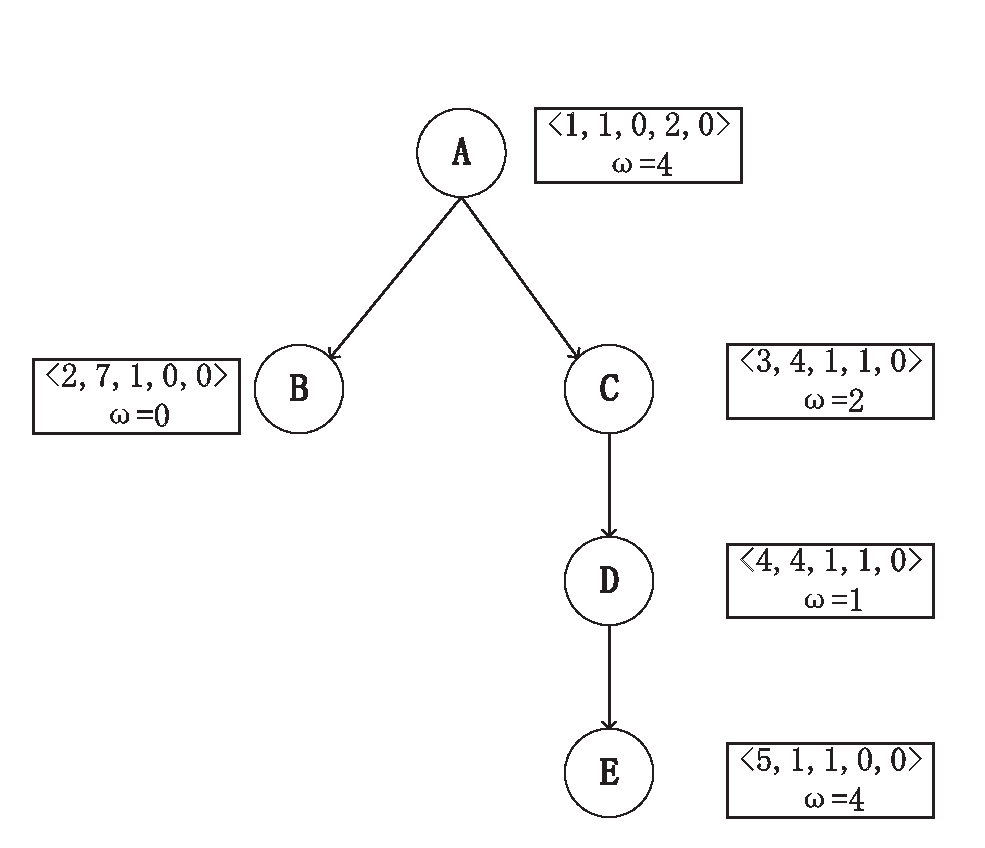
\includegraphics[width=8cm] {feature.eps}}
  \caption{\label{1}  An example of feature of 5UD-CFG}
\end{figure}

\subsection{Monotonicity of feature of 5UD-CFG} 
It is important to prove the monotonicity of the feature of the 5UD-CFG. The monotonicity shows the different CFGs have the different feature, at the same time, the same CFG has the same feature.  
\begin{proof}
	We use a expression to show the relationship between the edge set $E$ and the node weight set $W$, $W=f(E)$, the $f()$ is not a continuous function, is a discrete functions. If the $E_{CFG_j}=E_{CFG_k}$, the $W_{CFG_j} = W_{CFG_k}$. Exchanging condition and conclusion, it is also established. If the $W_{CFG_j} = W_{CFG_k}$, the $E_{CFG_j}=E_{CFG_k}$.
	
	Based on the Definition 3, the element in $W$, $\omega_j$ is calculated as follows:
	\begin{equation}
			\omega_j=\sum_{k\in j_o}(\omega_k +1),
	\end{equation}
	where the $j_o$ is the node-set of the outgoing degree of the node $j$. In a certain CFG, the $\omega_j$ of each node is determined by the iteration method. Therefore the $\omega_j~e_j$,is written by the $\omega_j=f(e_j)$. When the CFG is determined, the directed edges set $E$ of CFG is determined, therefore the node weight $\omega_j$ of each node is determined.
	
	Based on the Definition 2, we have
	\begin{equation*}
		\begin{split}
			& f_n=\frac{\sum_{j=1}^n \omega_j j e_j}{\omega}=\frac{\sum_{j=1}^n f(e_j) j e_j}{\omega}.\\
			& f_s=\frac{\sum_{j=1}^n \omega_j s_j e_j}{\omega}=\frac{\sum_{j=1}^n f(e_j) s_j e_j}{\omega}.\\
			& f_i=\frac{\sum_{j=1}^n \omega_j i_j e_j}{\omega}=\frac{\sum_{j=1}^n f(e_j) i_j e_j}{\omega}.\\
			& f_o=\frac{\sum_{j=1}^n \omega_j o_j e_j}{\omega}=\frac{\sum_{j=1}^n f(e_j) o_j e_j}{\omega}.\\
			& f_l=\frac{\sum_{j=1}^n \omega_j l_j e_j}{\omega}=\frac{\sum_{j=1}^n f(e_j) l_j e_j}{\omega}.\\
		\end{split}
	\end{equation*}
	
	We use reduction to absurdity to proof the monotonicity of feature of the 5UD-CFG. Assuming that there are two different CFGs' features are the same, therefore the $\omega$ is the same. And the following equations are the same.
	\begin{eqnarray*}
		\begin{cases}
			\sum_{j=1}^{n_1} f_1(e_{1j}) j e_{1j}=\sum_{j=1}^{n_2} f_2(e_{2j}) j e_{2j}\\	
			\sum_{j=1}^{n_1} f_1(e_{1j}) s_{1j} e_{1j}=\sum_{j=1}^{n_2} f_2(e_{2j}) s_{2j} e_{2j}\\
			\sum_{j=1}^{n_1} f_1(e_{1j}) i_{1j} e_{1j}=\sum_{j=1}^{n_2} f_2(e_{2j}) i_{2j} e_{2j}\\
			\sum_{j=1}^{n_1} f_1(e_{1j}) o_{1j} e_{1j}=\sum_{j=1}^{n_2} f_2(e_{2j}) o_{2j} e_{2j}\\
			\sum_{j=1}^{n_1} f_1(e_{1j}) l_{1j} e_{1j}=\sum_{j=1}^{n_2} f_2(e_{2j}) l_{2j} e_{2j}\\
			\sum_{j=1}^{n_1} f_1(e_{1j})=\sum_{j=1}^{n_2} f_2(e_{2j}).
		\end{cases}
	\end{eqnarray*}
	
	Before proving, we cite a existing lemma in the graph theory \cite{Feng} to prove the monotonicity of the feature of the 5UD-CFG.
	
	\begin{lemma}
		If the directed graph $G$ and the directed graph $G'$ are isomorphic,the input degree set $I$ and outgoing degree set $O$ of $G$, and the input degree set $I'$ and outgoing degree set $O'$ of $G'$ respectively are the same, $I=I'$ and $O=O'$. At the same time, the inverse is also true. 
	\end{lemma}
	
	We know the input degree set, the output degree set and the set of the number of loops in CFG $i, o, l$ is also determined by the edge set $E$. Based on the lemma 1, the edge set $E$ is also determined when the $i, o, l$ sets are determined. That is, if the input degree set of all nodes $i_{CFG_j} = i_{CFG_k}$ in a CFG, the $E_{CFG_j} = E_{CFG_k}$, if the outgoing degree set of all nodes $o_{CFG_j} =o_{CFG_k}$, the $E_{CFG_j}= E_{CFG_k}$ and if the $l_{CFG_j} = l_{CFG_k}$, the $E_{CFG_j}= E_{CFG_k}$. At the same time,  we know if the $W_{CFG_j} = W_{CFG_k}$, the $E_{CFG_j}= E_{CFG_k}$. Therefore, only if $n_1=n_2, e_{1j}=e_{2j}, f_1(e_{1j})=f_2(e_{2j}), j={1,2,...,n_1(n_2)}$, the equalities (1) are established.  
	Therefore, these two different CFGs actually are a same CFG. It does not exist two different CFGs have the same feature based on the proposed feature of 5UD-CFG.
\end{proof}

According to the above proof, we can know the proposed feature of 5UD-CFG is discrete monotonous. The different CFG has the different feature and the same CFG has the same feature. 

\section{Problem Description}
In this paper, we aim at the problem: \textit{How to achieve accuracy and scalability simultaneously in analyzing the app homology on Android Markets
?}

In order to obtain an effective app homology analysis strategy, we need to obtain an informative low-dimensional representation from the extracting CFG data. Refine such representation is a non-trivial task due to the following difficult points:
\begin{enumerate}
  \item Extracting the feature of CFG of app binary codes needs to preserve both characteristics of basic blocks and the call structure. Since CFG is a directed graph in most cases, and their corresponding vertexes have own unique features, which needs to be extracted from basic blocks. How can we carefully deal with such graph property in the representation learning process.
  %\item The ultimate goal is to train an app homology analysis system based on the learned representation of the CFG. If we can incorporate the analysis system training procedure into the representation learning process, the classifier process will indirectly interact with the original CFG via latent factors. How can we effectively fuse these two procedures together to achieving the accurate and scalability the app homology analysis?  
  \item The mass quantity of apps have the millions and billions CFG features that leads to the scalable graph match problem. Graph match essentially is a NP-problem. We need to find a practicable approach to accurately reduce CFG features. Moreover, the availability of the reducing feature should be proved theoretically and practically.
  \item The rapidly increasing novel apps cause the previous feature data that should be updated timely. Since if app samples are changed, the feature data also needs to be re-obtained. We need to find a incremental computation algorithm that just needs to compute the novel app features excluding pervious app features.   
\end{enumerate}
%\subsection{Problem Formulation}

To address those critical problems, we extract the numeric and structural features in the binary code of Android apps based on the following basic definition. %We formally define the problem of large-scale app homology analysis using the CFG extraction with basic-block feature, the first-hierarchy CFG embedding model considering the first-order call structure of CFG and the second-order call structure of CFG, and the second-hierarchy embedding tensor model based on the first-hierarchy embedding CFGs' feature vector. 
   
\textbf{Definition 1.} \emph{(CFG extraction with the basic block feature)}. We extract CFG that each vertex is with five unique feature called 5UD-CFG, is a directed graph $G=<V,E>$, where $V$ is a set of basic blocks in a function;$E \subseteq V \times V$ is a set of edges representing connections between these basic blocks. Each vertex has a unique feature with five numeric elements based on the statistical features of basic blocks. The corresponding feature of a vertex represents as a vector $v=\vec{x} =<num, ~squ, ~in, ~out, ~loop>$. $num$ is the sequence number of the basic block in the CFG, $squ$ is the number of opcodes for a basic block, $in$ is the number of calls, $out$ is the number of basic blocks that is called by other vertexes, $loop$ is the number of loops of a vertex. Each vertex has a unique weight $\omega \in \aleph$. Fig.1 (a) shows a real extracting CFG.


%\begin{figure}[hbt]
%  \center{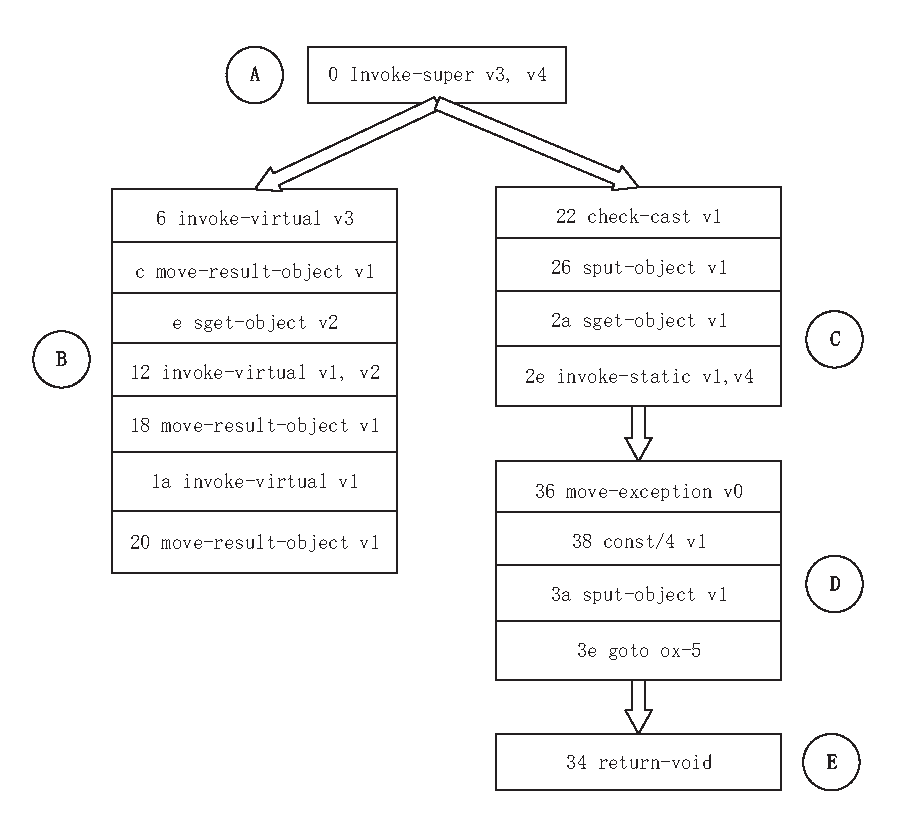
\includegraphics[width=8cm] {realcfg.eps}}
%  \caption{\label{1}  An example of real CFG}
%\end{figure}

Given a set of training CFGs $C=[c_1,~c_2,~...,~c_{N_T}]\in R^{m\times 5\times N_T}$ where $c_i \in R^{m \times 5}$ is a CFG, $m$ is the number of vertexes in a CFG, and $N_T$ is the number of all CFGs. Embedding aims to map the graph data into a low-dimensional latent space, where combines all vertexes of a CFG represented as a low-dimensional vector. As this explained, both vertex features and the graph structure are essential to be preserved.Then we define the first-hierarchy 5UD-CFG embedding model.

\textbf{Definition 2.} \emph{(First-hierarchy 5UD-CFG embedding)} Given a CFG that each vertex has five eigenvalues denoted as $G=(V, E)$, CFG embedding aims to learn a mapping function $f: \sum_1^m \vec{x_i} \mapsto y_i \in R^d$, where $d<< |V|.$ The objective of function is to distinguish the similarity between the feature of a CFG $y_i$ and the feature of another CFG $y_j$, explicitly preserve the first-order and second-order call structure of $v_i$ and $v_j$. We denote the result of first-hierarchy CFG embedding as 5UD-CFG.

We consider the \emph{first-order call structure} and the \emph{second-order call structure} to show CFG structure based on the definition of the first-hierarchy 5UD-CFG embedding.

%\begin{Definition}
\textbf{Definition 3.} \emph{(First-Order Call Structure)} The first-order call structure describes the directed pairwise structure between vertexes. For any pair of vertexes, if $l_{i,j}=1$, there exists an directed first-order call structure between the vertex $v_i$ and $v_j$.  Otherwise, the first-order call structure between the vertex $v_i$ and $v_j$ is 0.
%\end{Definition}

The first-order call structure is necessary for the CFG embedding to imply the first-order inherit or invocation between two real basic blocks in real binary codes. The result of the basic block will be directed used by the directional vertexes.

%\begin{Definition}
	\textbf{Definition 4.} \emph{(Second-Order Call Structure)} The second-order call structure between a pair of vertexes describes the call structure of neighborhoods. Let $N_u={l_{u,1}~,~...,~l_{u,|V|}}$ denote the first-order call structure between $v_u$ and other vertexes. $|V|$ is the number of neighborhoods. The second-order call structure is determined by the similarity of $N_u$ and $N_v$. 
%\end{Definition}

Intuitively, the second-order call structure assumes that if two vertexes share many common basic blocks, they may have more connections. Such an assumption has been proved reasonable in many fields \cite{TangQWZYM15}. A father basic block is most frequently called in other basic blocks.


\textbf{Definition 5.} \emph{(Second hierarchy embedding tensor model)} To represent all CFGs' features of all apps, the proposed tensor embedding model can be written as a three-order tensor model $A^{I_f*I_c*I_1}$, which $I_f, I_c$ indicate the feature vector of CFG and the number of all CFGs. For embedding CFG, $I_f=5$ and $I_c=tn$, $tn$ is the total training number of CFGs. $tn$ can be expanded with the development of apps. $I_1$ is the label of the app. Using the label $I_1$, we can partition app communities that can be easier used for the app homology analysis.
%\subsection{Problem Overview}
% the following steps: starting with a unknown app in binary code. We are searching for binaries containing the similarity functions in known app features' database. We extract the unique feature vector for each function in app. Then we handle with all extracting CFG features to achieving an effective and scalable homologous app search.

%\begin{Definition}


\section{Solution Overview}
In this section, we present the key idea of our solution to the app homology embedding problem, which can be scalable and accurate. In our approach, we show binary codes of app represented by 3TU-CFG. 

We propose the two-hierarchies embedding mapping model for the extracting CFG from app's binary codes. The two hierarchies embedding model satisfy several highlights: first, it extracts the CFG that each vertex has five unique eigenvalues. This CFG with feature is referred to the raw feature, from a decompiling binary function of app. It remains characteristics of raw binary code of app. Second, the first-hierarchy 5UD-CFG embedding is able to preserve both the \emph{first-order call structure} and the \emph{second-order call structure} between vertices of CFG. Third, the second-hierarchy tensor embedding can handle the scalable and considerable CFG feature data, say millions and billions apps' homology detection in very short time. 

The proposed methods including the following main steps, as shown in Fig. 2: 1) \emph{original CFG extraction with vertex features}, 2) \emph{5UD-CFG embedding feature vector generation}, 3) \emph{3TU-CFG tensor embedding compressing and clustering}, 4) \emph{3TU-CFG tensor embedding update}. The first step and the second step are the first-hierarchy embedding process. They aim at extracting the original control flow graph that each vertex of CFG has five eigenvalues, and embedding them into a monotonous feature vector (Section 4). The third step and the fourth step are the second-hierarchy embedding process. They use the tensor factorization learning algorithm to further embed the feature vector that is generated by the first-hierarchy embedding process to a more low-dimensionality feature vector, and this model also provide an incremental feature data update approach (Section 5). Finally, given a app, we use the KNN \cite{ChandrasekaranD18} to find its most similarity app in feature data. Since each app is decompiled into several functions, and each function is embedded into a low-dimensionality unique and accurate feature vector in two hierarchies embedding process. We can directly apply fast KNN search \cite{AntolD17} to conduct efficient matches and searches. The detailed of each steps will be discussed in the following section.

In the first-hierarchy 5UD-CFG embedding process, we show the monotonicity of 5UD-CFG feature vector, which give a high scalability and accurate. When a function changes a little, its 5UD-CFG will not change a lot. Make sure two similarity apps have a little different, and two different apps have a large different. In the second-hierarchy 3TU-CFG learning embedding process, we show the embedding reversibility and the monotonicity of 3TU-CFG, which generates a more concise embedding feature vector to monotonously map the original apps' function. The compress and clustering algorithm based on the tensor embedding model give a further significant scalability and accurate. Moreover, the tensor computations make the feature data updated easier in the second-hierarchy tensor embedding process. 

\begin{figure*}[!hbt]
   \centering
   \subfigure[]{\label{fig: 1}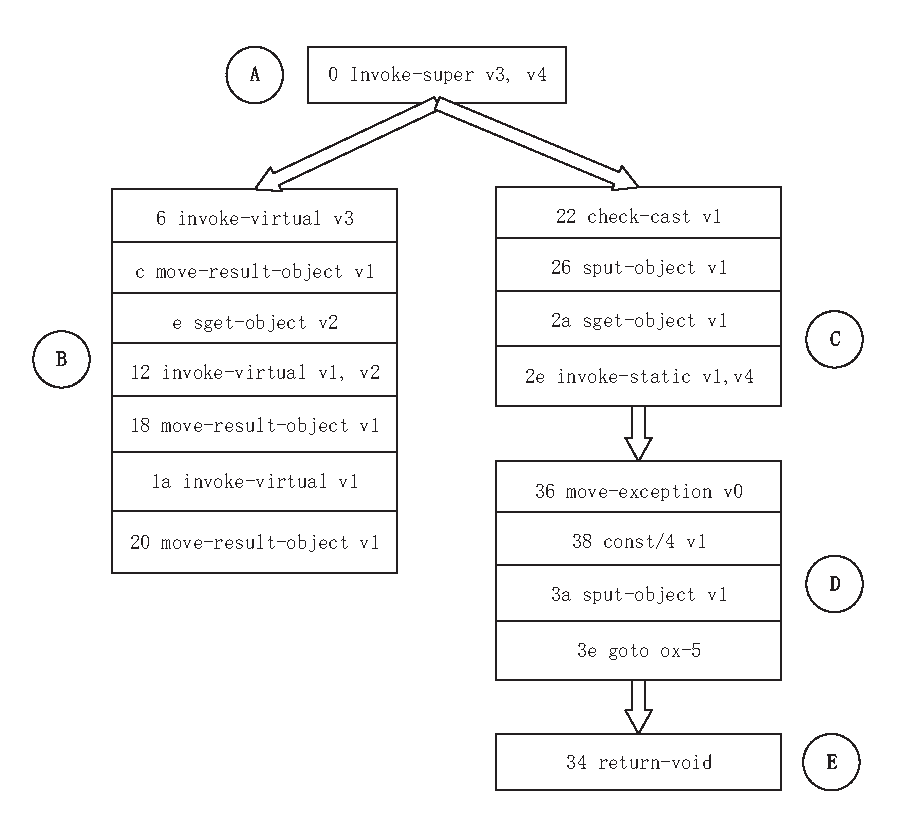
\includegraphics[width=0.30\textwidth]{realcfg.eps}}
   \hspace{0.1in}
   \subfigure[]{\label{fig: 2}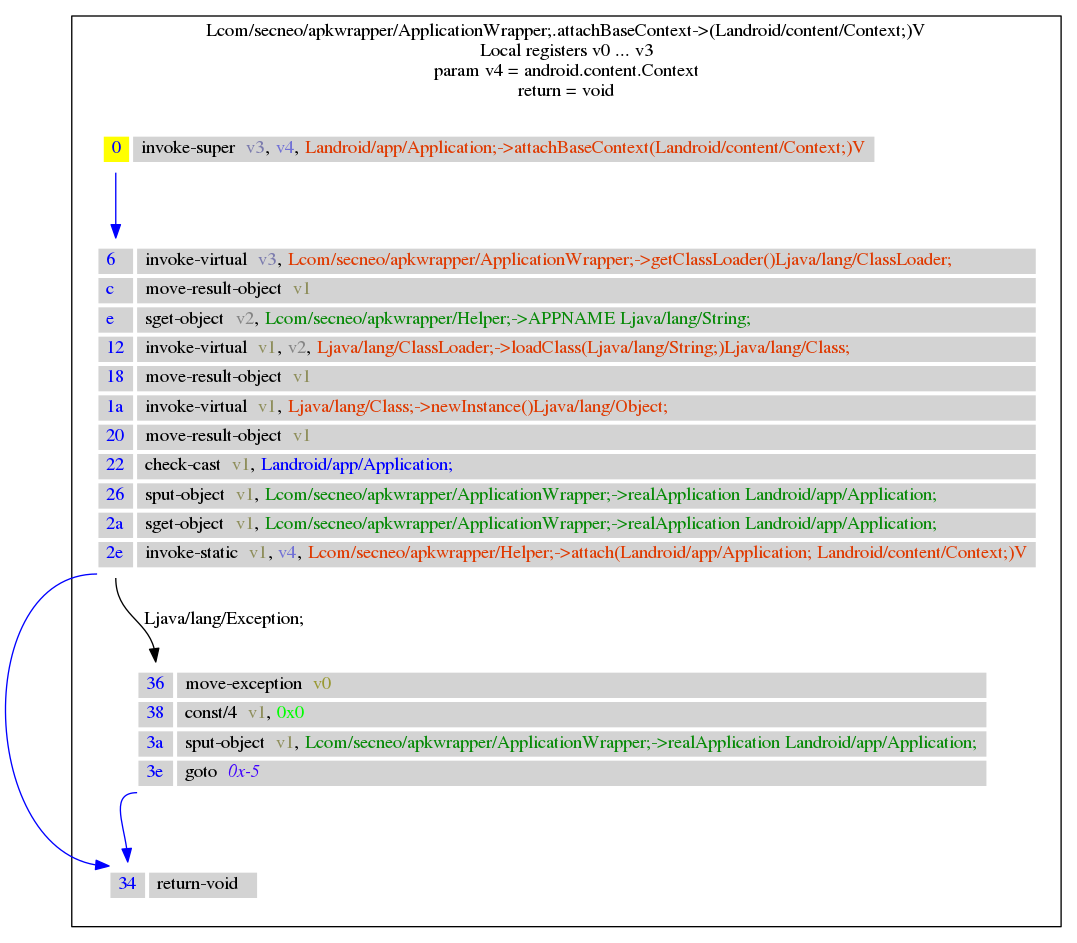
\includegraphics[width=0.30\textwidth]{cfgexample.png}} \hspace{0.1in}
   \subfigure[]{\label{fig: 3}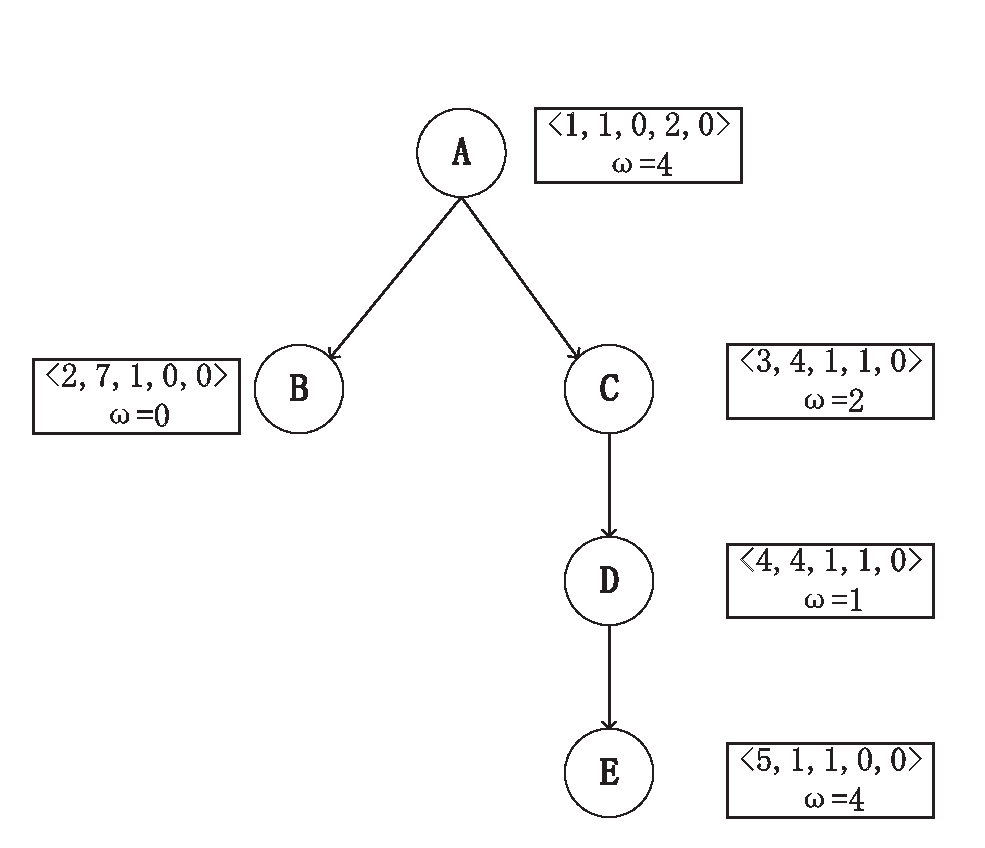
\includegraphics[width=0.30\textwidth]{feature.eps}}\\
   \caption{(a) shows an example of real CFG; (b) shows extracting CFG with the basic block; (c) shows an example of CFG with embedding feature; (a) is used in this Section 3, (b) and (c) are used in Section 5. }
   \vspace{-3 mm}
   \end{figure*}
   
   \begin{figure*}[!hbt]
  \center{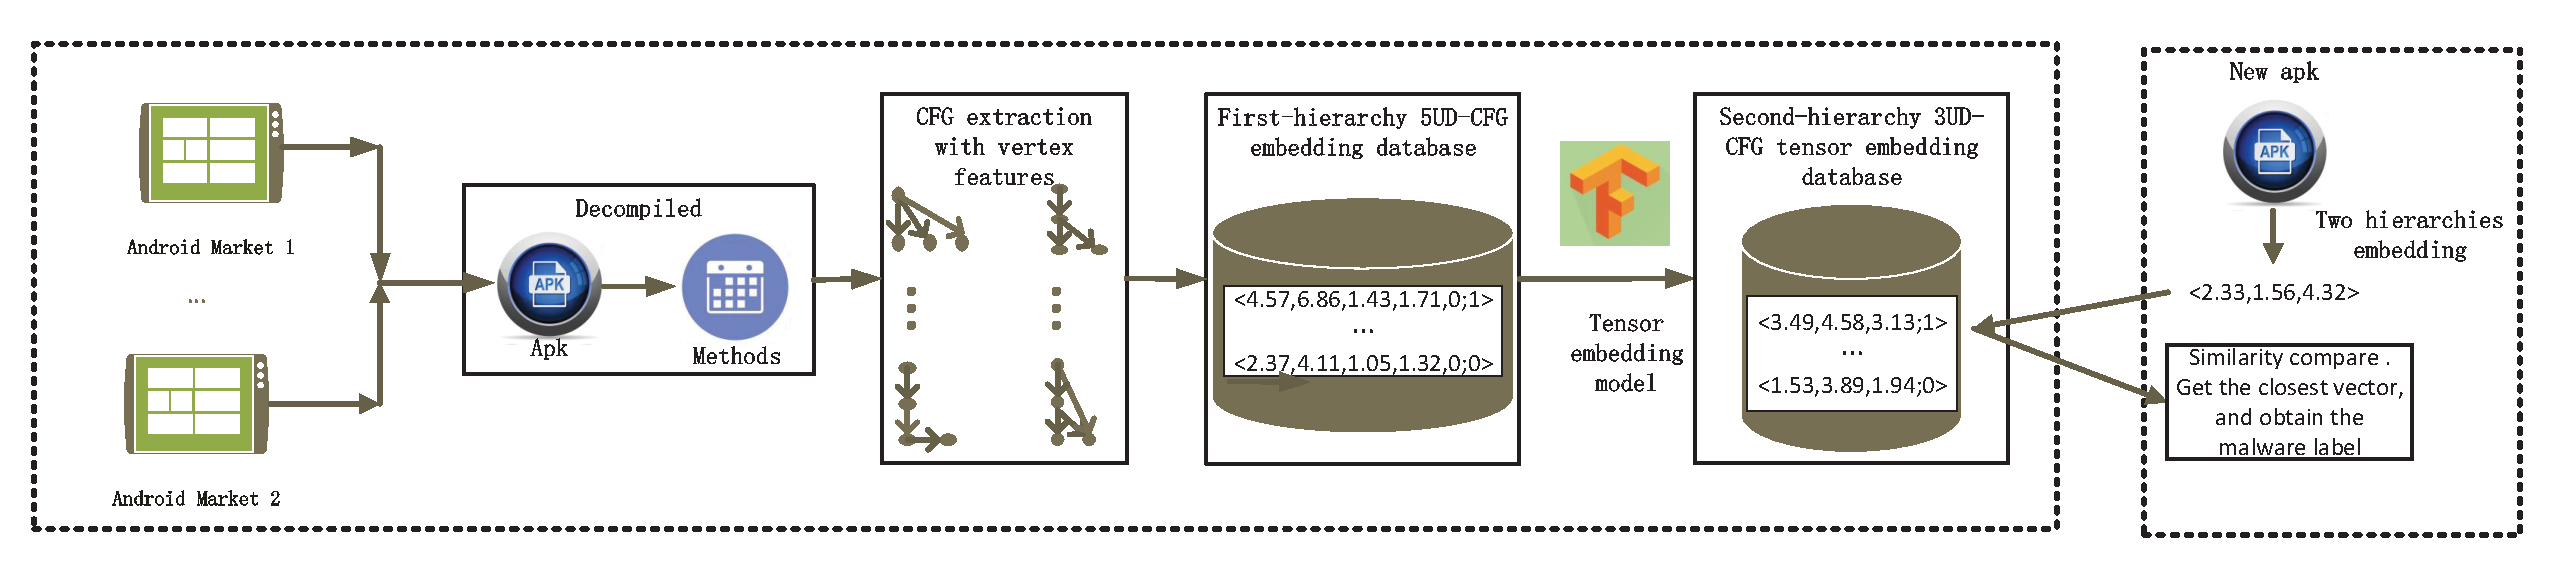
\includegraphics[width=18cm] {overview.eps}}
  \caption{Overview}
\end{figure*}
                                                                                                                                                                                                                                                                                                                                                                                                                                                                                                                                                                                                                                                                                                                                                                                                                                                                                                                                                                                                                                                                                                                                                                                                                                                                                                                                                                                                                                                                                                                                                                  
\section{First-hierarchy 5UD-CFG embedding model}
In this section, we propose the detailed approaches how the model generates 5UD-CFG from Android apps. The traditional CFG is the common feature used in bug search. Moreover, different from other attributes on basic blocks, such as I/O pairs and statics features \cite{EschweilerYG16} \cite{PewnyGGRH17}, are more accuracy matching. Following the idea of the traditional CFG extraction, this paper utilizes CFG with different basic block level attributes with five eigenvalues called 5UD-CFG. We also prove the monotonicity of 5UD-CFG, a 5UD-CFG vector represents a CFG.


%\subsection{Disassembly of Android Application and original CFG extraction}
%In our system, the pretreatment of an application consists of disassembling the application and extracting opcode sequences. A code file is a dex file that can be transformed into smali files, where each smali file represents a single class and contains methods of such a class. Each method contains instructions and each instruction consists of a single opcode and multiple operands.  
%
%After preparation, including downloading all apps from multiple markets and extracting methods from the apps, we encode a projection form of CFG to get the unique feature of the function of an app.
%
%CFG is the control flow graph of a method. Each vertex in a CFG corresponds to a basic block in the method. A basic block is a straight-line piece of code with one entry point and one exit point. Jump targets start a block, and jump end a block. Directed edges are used to represent jumps in the control flow.
%
%Before discussing the CFG embedding, we extract the feature of basic block for each vertex in a CFG. 

Fig. 1(b) shows a primitive extracting CFG from a function. A vertex represents a basic block, and a edge represents a call link between two basic blocks. A basic block is a set of opcodes. The outgoing edges of a vertex $A$ represents the basic block $A$ is called by other basic blocks. The input edges of a vertex $A$ represent the the basic block $A$ calls other basic blocks. 

%\begin{figure}[hbt]
%  \center{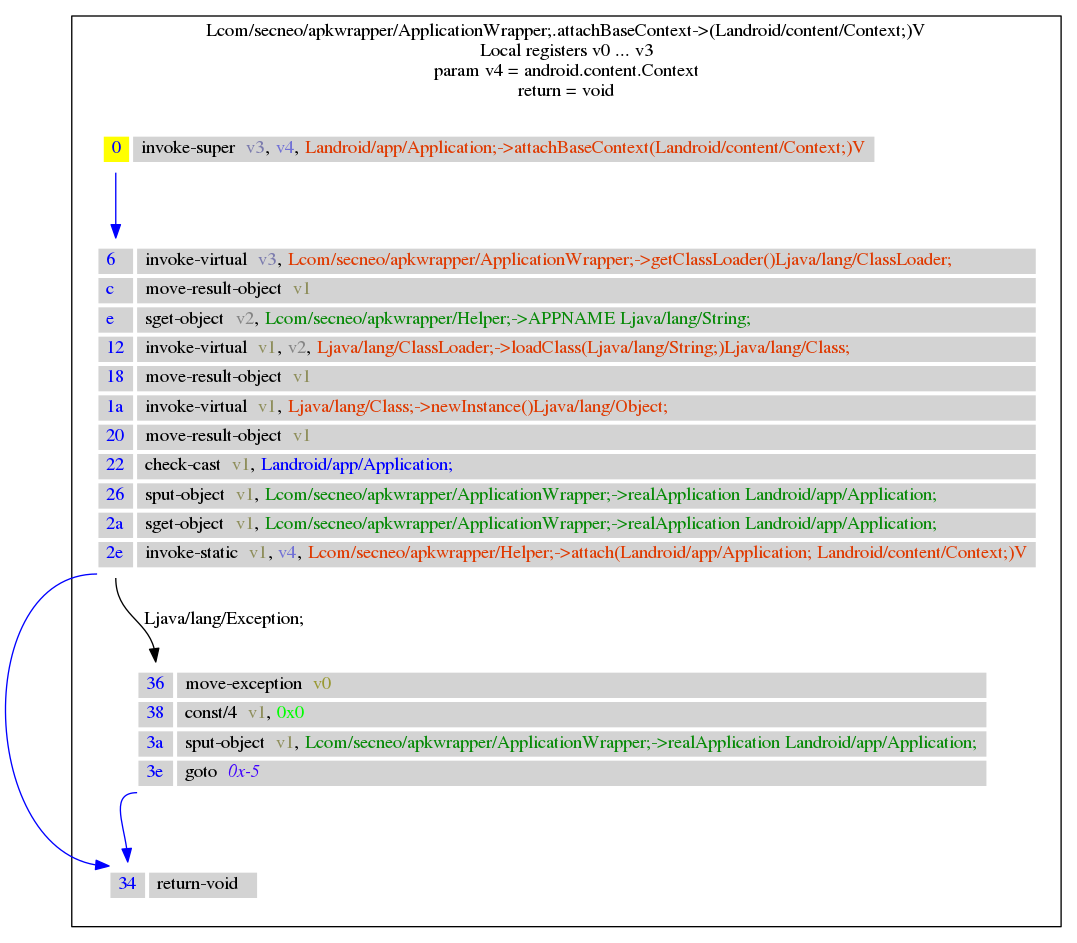
\includegraphics[width=8cm] {cfgexample.png}}
%  \caption{An example of a method CFG in a real apk}
%\end{figure}

%\subsection{Notation} 
%Before introducing the CFG embedding model, we define some of the terms and notations in Table 1 which will be used later. 
%\begin{table}[!htb]
%\newcommand{\tabincell}[2]{\begin{tabular}{@{}#1@{}}#2\end{tabular}}
%\caption{Propagation model}
%\centering
%\begin{tabular}{|l|l|}
%\hline
% Symbol& Definition \\
% \hline
% n & number of vertexes \hline
% V & vertex set of CFG\hline
%& $0.2,~ 0.5,~ 1$\\
%\hline
%The {\color{black}recovery} probability & $\mu$ & $0, ~0.5, ~1$\\
%\hline
%\tabincell{l}{The influence factor\\ of the search engine} & $\xi$ & $0.2, ~0.5,~ 1$\\
%\hline
%\tabincell{l}{The growth velocity\\ of susceptible vertexes} & r & 0.5\\
%\hline
%\tabincell{l}{The disappearing velocity\\ of susceptible vertexes} & d & 0.1\\
%\hline
%\tabincell{l}{The vanishing velocity \\ of the influence \\by the search engine} & c & 0.1\\
%\hline
%\end{tabular}
%\end{table}}

%\subsection{5UD-CFG embedding}

The main idea of 5UD-CFG embedding is to encode a CFG as a 5-dimensional vector. We use a generic nonlinear mapping to update the embedding result based on the CFG topology. 
%A new round of embedding process will start after the embedding update for all vertexes in the pervious round. 
%\end{Definition}

A 5UD-CFG can be viewed as a set of vertexes connected by edges based on the CFG topology. We need to train the vertex weight of each vertex (basic block). The vertex weight of each vertex is used to combine all vertex for representing the CFG. The embedding vector monotonously represent the CFG. We define the feature of a 5UD-CFG based on the 3D-CFG \cite{ChenLZ14}.

\textbf{Definition 6.} The feature of 5UD-CFG is a vector $<f_n, f_s, f_i, f_o, f_l>.$
\begin{equation*}
	\begin{split}
	& f_n=\frac{\sum_{e(j,k)\in CFG}(\omega_jn_j+\omega_kn_k)}{\omega},\\
	& f_s=\frac{\sum_{e(j,k)\in CFG}(\omega_js_j+\omega_ks_k)}{\omega},\\
	& f_i=\frac{\sum_{e(j,k)\in CFG}(\omega_ji_j+\omega_ki_k)}{\omega},\\
	& f_o=\frac{\sum_{e(j,k)\in CFG}(\omega_jo_j+\omega_ko_k)}{\omega},\\
	& f_l=\frac{\sum_{e(j,k)\in CFG}(\omega_jl_j+\omega_kl_k)}{\omega},\\
	& \omega=\sum_{e(j,k)\in 5UD-CFG}(\omega_j+\omega_k).\\	
	\end{split}
\end{equation*}
 where $e(j, k)$ is an edge in CFG. This edge connects two vertexes $j$ and $k$. 

The key factor of feature vector of the 5UD-CFG embedding is the vertex weight $\omega$, and we need to show the monotonicity of 5UD-CFG. For each directed edge $(i,~j)$ in CFG, we define the joint probability of the first-order call structure between vertex $v_i$ and vertex $v_j$ as follows:
\begin{equation}
  Link_1(v_i,~v_j)=\frac{1}{1+exp(\vec{x_i}^T \vec{x_j})},
\end{equation}
where $\vec{x_i} \in R_d$ is feature vector of vertex $v_i$, $\vec{x_i}=~<num_i,~squ_i, ~in_i, ~out_i, ~loop_i>$. In Eq.(1), we use the sigmod function as the embedding activation function. Eq.(1) defines a joint probability distribution of the vertex call over a CFG, and its empirical probability of two vertexes can be defined as $\widehat{Link_1}=\frac{\omega_j}{\omega_i\times W}$, where $W=\sum_{i\in V} \omega_i$ is related with the number of vertexes that call the vertex $v_i$ by the first-order call structure. To preserve the first-order call structure, we use the distance between two probability distributions to be the objective function. A straightforward way is to minimize the following objective function:
\begin{equation}
	 y_i^{(1)}=d~(\widehat{Link_1}, ~Link_1),
\end{equation}
where $d(.,.)$ is the distance between two distributions. We minimize the KL-divergence \cite{TangQWZYM15} of two probability distributions. Therefore, the objective function is:
\begin{equation}
	y_i^{(1)}=-\sum_{(i,j)\in E} s_{i,j}~ log~ Link_1~(\omega_i  v_i, ~\omega_j v_j).
\end{equation}

The second-order call structure assumes that the basic block (vertex) are invoked by the another vertexes exclude neighbors. Each basic block is also treated as a specific "contexts" of other vertexes. We define the joint probability of the second-order call structure between vertex $v_i$ and vertex $v_j$ as follows:
\begin{equation}
  Link_2(v_j|v_i)=\frac{exp(\vec{x_j}^T \vec{x_i})}{\sum_{k=1}^{|V|} exp(\vec{x_k}^T \vec{x_i})},
\end{equation}
where $|V|$ is the number of other vertexes exclude neighbor vertexes. To preserve the second-order call structure, we need to make the 
conditional distribution of  ``contexts" closed to the empirical distribution $\widehat{Link_2}~(v_j|v_i)=\frac{\omega_j}{\omega_i \times d_i}$,  where $d_i$ is the degree of vertex $i$. Therefore, we minimize the following objective function:
\begin{equation}
	 y_i^{(2)}=\sum_{i\in V}~d_i d(\widehat{Link_2},~ Link_2),
\end{equation}
where $d(.,.)$ is the distance between two distributions. We minimize the KL-divergence \cite{TangQWZYM15} of two probability distributions. Therefore, the objective function is as follows:
\begin{equation}	
	y_i^{(2)}= -\sum_{(i,j)\in E} l_{i,j}~ log~ Link_2~((\omega_j v_j) | (\omega_i v_i)),
\end{equation}
where $l_{i,j}$ is the connection between vertex $v_i$ and vertex $v_j$. If $l_{i,j}=1$, there exists a edge from vertex $i$ to $j$. If $l_{i,j}=-1$ for vertex $i$, there exists an edge from vertex $j$ to $i$. Otherwise there is no directed edge between $v_i$ and $v_j$.

To generate the CFG feature vector by preserving both the first-order and second-order call structure, we train parameters $\omega_i$ for each vertex. We adopt Maximum Likelihood Estimate for optimizing Eq (3) and (6). We sample all edges $(i,j)$ in a CFG, the gradient of weight of vertex with embedding vector $\vec{x_i}$ will be calculated as:
\begin{equation*}
	\begin{split}
	& \nabla_1 =\frac{\partial y_i^{(1)}}{\partial \omega_i}=\frac{\partial (-\sum_{(i,j)\in E} s_{i,j}~log ~Link_1(\omega_i v_i, ~\omega_j v_j))}{\partial \omega_i}\\
	& \nabla_2 =\frac{\partial y_i^{(2)}}{\partial \omega_i}=\frac{\partial (-\sum_{(i,j)\in E} s_{i,j}~log~ Link_2((\omega_j v_j) | (\omega_j v_j) ))}{\partial \omega_i}.\\
	\end{split}
\end{equation*}

%说明由于d是两个分布之间的距离,然后那个p的平均值就是empricial distribution 是wi/wj,这两个是绝对不相同,只要那个训练的向量靠近这个值,说明绝对是递增的,只用这么训练就可以了后面举个例子。
 The embedding vector space of all vertexes in a CFG is spanned by the vertex weight $W$. 
 
 In our case, we only need to ensure that it is monotonicity to embed a CFG as a vector. The gradient is used to calculate the distance between two probability distributions between original $link_{\left\{1~or~2\right\}}$ and embedding $\widehat{link_{\left\{1~or~2\right\}}}$. From Eq. (2) and Eq. (4), we know that original $link_{\left\{1~or~2\right\}}$ is monotonous. When the gradient $\nabla_1+\nabla_2 \rightarrow 0$, $link_1\approx \widehat{link_1}$ and $link_2\approx \widehat{link_2}$. The $link_1$ and $link_2$ are monotonous, so the embedding $\widehat{link_1}$ and $\widehat{link_2}$ are monotonous and $W=[\omega_1,~...,~\omega_n]$ are monotonous. Therefore, for ensuring the monotonicity of the embedding vector, we combine the gradient $\nabla=\nabla_1+\nabla_2 =0$ by the Maximum Likelihood Estimate formulas. 
 let
 \begin{equation*}
	\begin{split}
	& \frac{\partial y_i^{(1)}}{\partial \omega_i} +\frac{\partial y_i^{(2)}}{\partial \omega_i}= 0, \\
	\end{split}
\end{equation*}
 we train the parameter of the vertex weight sequence $W=[\omega_1,~\omega_2,~...,~\omega_n ] mod (n-1)$, where $n$ is the number of nodes in the CFG.

%we give an example to show how to calculate the $\omega_i$. vertex $A$ with the first sequence number is called by the vertex $B$ and the vertex $C$ directly. vertex $C$ is called by the vertex $D$ directly, and vertex $D$ is called by the vertex $E$ directly. This outgoing degree of vertex $A$ is $A_{\searrow B}^{\nearrow C \longrightarrow D \longrightarrow E}$. $A$ is related with $B$, $C$, $D$ and $E$. The result of vertex $A$ will be passed to vertex $B$ and vertex $C$. This process will also influence the vertex $D$ and $E$ by influencing the vertex $C$. 

Form above analysis, we know that the vertex weight $\omega_j$ is trained by the CFG topology $\sum_{e(j,k)\in 5UD-CFG}$, which is unique when the CFG is determined. As the view of the Definition 6, $<f_n, ~f_s, ~f_i, ~f_o, ~f_l>$ is related with $\sum_{e(j,k)\in 5UD-CFG}$. The different CFG has the different vertex weight sequence $W$. Therefore, they have different embedding vector. Fig.1 (c) shows an example of CFG that contains embedding parameters and basic blocks with features. There is an example for computing 5UD-CFG, which is shown in the appendix.

%\subsection{An example of 5UD-CFG embedding}
%we give an example to show how to calculate $\omega_i$. As shown in the Fig. 1 (c), vertex $A$ with the first sequence number is called by the vertex $B$ and the vertex $C$ directly. The vertex $C$ is called by the vertex $D$ directly, and vertex $D$ is called by the vertex $E$ directly. This outgoing degree of vertex $A$ is $A_{\searrow B}^{\nearrow C \longrightarrow D \longrightarrow E}$. $A$ is related with $B$, $C$, $D$ and $E$. The result of vertex $A$ will be passed to vertex $B$ and vertex $C$, which have a first-order call structure with vertex $A$. This process will also influence the vertex $D$ and $E$ by influencing the vertex $C$, which are the second-order call structure. 
%%\begin{figure}[hbt]
%%  \center{\includegraphics[width=8cm] {cfg.eps}}
%%  \caption{\label{1}  An example of real CFG}
%%\end{figure}
%
%Based on the above first-order call structure and the second-order call structure, the particular trained process of $W$ is as follows:
%
%\begin{eqnarray*}
%	\begin{cases}
%		\frac{\partial~Link_1^{(1)}}{\partial~\omega_1} +\frac{\partial~Link_2^{(1)}}{\partial~\omega_1}=0\\
%		\frac{\partial~Link_1^{(2)}}{\partial~\omega_2} +\frac{\partial~Link_2^{(2)}}{\partial~\omega_2}=0\\
%		\frac{\partial~Link_1^{(3)}}{\partial~\omega_3} +\frac{\partial~Link_2^{(3)}}{\partial~\omega_3}=0\\
%		\frac{\partial~Link_1^{(4)}}{\partial~\omega_4} +\frac{\partial~Link_2^{(4)}}{\partial~\omega_4}=0\\
%		\frac{\partial~Link_1^{(5)}}{\partial~\omega_5} +\frac{\partial~Link_2^{(5)}}{\partial~\omega_5}=0.\\
%		%\omega=4+0+2+1+0=7.
%	\end{cases}
%\end{eqnarray*}
%
%let $log(1+exp \left\{ k\times \omega_i \times \omega_j \right\} )=k\times \omega_i \times \omega_j$ and the weight of final vertex $\omega_5=0$, we have
%\begin{eqnarray*}
%	\begin{cases}
%		9\omega_2+10\omega_4+6\omega_5=0 \\
%		35\omega_3+37\omega_4+18\omega_5-18\omega_1=0 \\
%		20\omega_5+35\omega_2-18\omega_1=0 \\
%		25\omega_5+37\omega_2+10\omega_1-60\omega_3=0 \\
%		20\omega_3+6\omega_1+18\omega_2-50\omega_4=0 \\
%		W={\omega_1, \omega_2,\omega_3,\omega_4,\omega_5 }~mod~4.
%	\end{cases}
%\end{eqnarray*}
%
%We obtain the $W=[1,~2,~3,~1,~0].$
%
% Based on the Definition 6, we calculate the feature of a 5UD-CFG as follows:
%\begin{eqnarray*}
%	\begin{cases}
%	    \omega=1+2+3+1+0=7. \\
%		f_n=\frac{1\times 2\times 1+ 2\times 1\times 2+3\times 2\times3+ 4\times 2\times 1 +5\times 1 \times 0}{1+2+3+1+0}=4.57\\
%		f_s=\frac{1\times 2\times 1+ 7\times 1\times 2+4\times 2\times3+ 4\times 2\times 1 +1\times 1 \times 0}{1+2+3+1+0}=6.857\\
%		f_i=\frac{0\times 2\times 1+ 1\times 1\times 2+1\times 2\times3+ 1\times 2\times 1 +1\times 1 \times 0}{1+2+3+1+0}=1.429\\
%		f_o=\frac{0\times 2\times 1+ 2\times 1\times 2+1\times 2\times3+ 1\times 2\times 1 +0\times 1 \times 0}{1+2+3+1+0}=1.714\\
%		f_l=\frac{0\times 2\times 1+ 0\times 1\times 0+0\times 2\times2+ 0\times 2\times 1 +0\times 1 \times 0}{1+2+3+1+0}=0.\\
%		
%	\end{cases}
%\end{eqnarray*}


%\begin{figure}[hbt]
%  \center{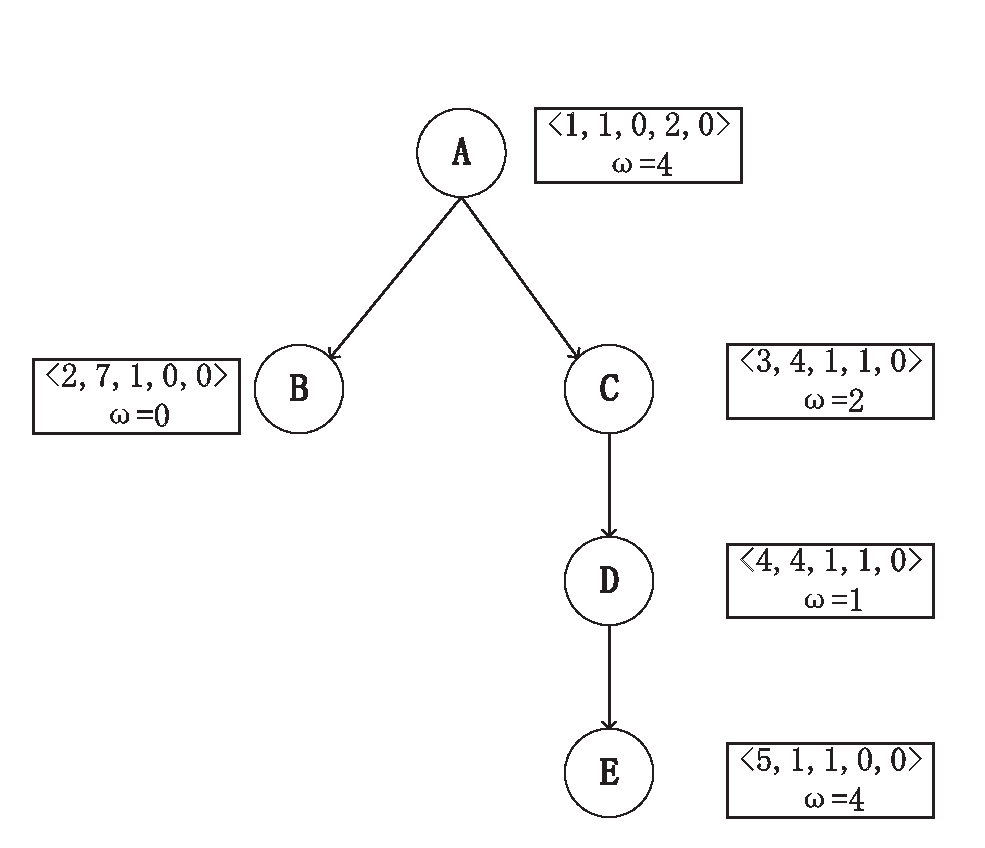
\includegraphics[width=8cm] {feature.eps}}
%  \caption{\label{1}  An example of feature of 5UD-CFG}
%\end{figure}

\section{Second-hierarchy Tensor Embedding model} 

According to the extracting 5UD-CFG in the Section 4, this section discusses how we utilize the feature vector of 5UD-CFG embedding, compress and cluster them into a more concise feature that is suitable for achieving scalable and accurate app homology analysis. The second-hierarchy embedding process is the tensor embedding, which generates 3UD-CFG based on 5UD-CFG. 

\subsection{Tensor embedding model}
We propose a tensor embedding model for generating a more concise and effective feature vector. We review a well-studied factorization and compact model that are based on the first-hierarchy CFG embedding. In Definition 5, we can set $I_1$ of the second-hierarchy embedding tensor model firstly. For example, if the tensor embedding model is used to malware detection, we can set $I_1$ as the malware label of the app, $I_1$ can be defined as \emph{$I_1=1$ if this method is from the begin app, $I_1=0$ if this method is from the malware app,}
%Relationships among the number of CFG, the feature of CFG and the classification of CFG. 
%\begin{equation*}
% \begin{split}
%&I_1=\\
%\begin{matrix}
%1,~ if this method is from the begin apk\\
%0,~ if this method is from the malware apk \\
%\end{matrix}
%\end{split}
%\end{equation*}

%\begin{eqnarray*}\label{nn}
%\begin{cases}
% &I_1=1,~ if~this~method~is~from~the~begin~apk,\\
% &I_1=0,~ if~this~method~is~from~the ~malware~ apk.\\
%\end{cases}
%\end{eqnarray*}

%\begin{eqnarray*}
%	\begin{cases}
%		I_1=& 1, if this method is from the begin apk\\
%		& 0, if this method is from the malware apk.
%	\end{cases}
%\end{eqnarray*}

We use the accepted notation where an order-3 tensor is indexed by 3 indices and can be represented as a multidimensional array of data \cite{Kilmer2011Factorization}. That is, an order-3 tensor, $A$, can be written as 
\begin{equation}
	A=(a_{i_1i_2i_3})\in R^{n_1\times n_2\times n_3}~~(n_3=1).
\end{equation}

A third-order tensor can be pictured as a "cube" of data. It is convenient to refer to its slices. We use lateral slices to specify which two indices are held constant. Using the MATLAB notation, $A(:,k,1)$ corresponds to the k-th lateral slice. $A$ tube of a third-order tensor is defined by holding the first two indices fixed and varying the third. In particular, the third orientation of our tensor embedding model indicates a label. It does not join in the calculation of the tensor embedding model. 

As shown in the Fig. 3, we cut slices for the tensor embedding model expand in the horizontal orientation. 
\begin{figure}[hbt]
  \center{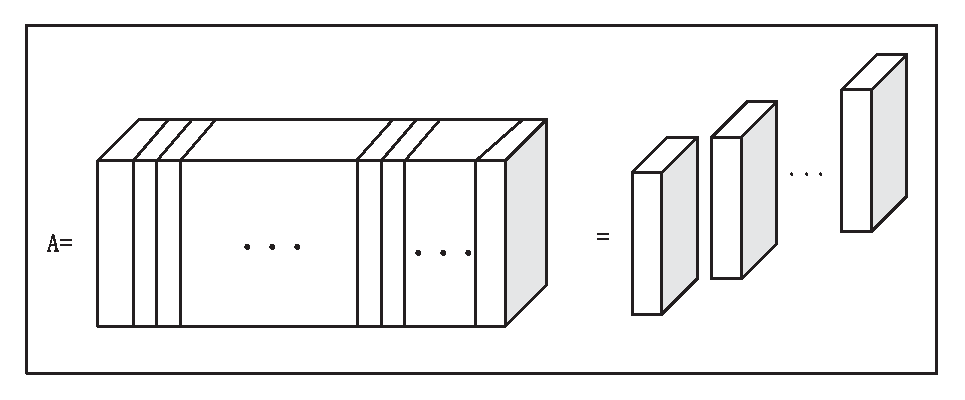
\includegraphics[width=8cm] {tensor.eps}}
  \caption{\label{1} Lateral slices of the tensor model $A$}
\end{figure}

For the third-order tensor embedding model, $A \in R_{n_1\times n_2 \times n_3}$, we have the representation that the tensor unfolding $A_{(3)}\in R^{I_f\times (I_n*1)}$ contains element $t_{i_1i_2}$ at the position with row number $f_i$ and column number $n_i$, $i_1$ is No. of the feature vector with five eigenvalues. $i_2$ is No. of the CFG. 

The following section, we will discuss how the function is decomposed in the tensor embedding model. 

\subsection{Compact 5UD-CFG to 3UD-CFG Based on tensor embedding model}
First we review the Singular Value Decomposition (SVD) \cite{Thomasian15} \cite{HanWZY18} as compressing algorithm for 5UD-CFG. An SVD of the tensor model that consists of all apps' 5UD-CFG embedding vector is $A=UDV^T$. We interpret the matrix $U$ to consist of latent embedding vectors in rows, for each entity represented in the first dimension of $A$. The matrix $A$ is constructed by a linear combination of the embedding $U$ with weights defines as rows of $(DV^T)^T$.

Then we consider $U=A(DV^T)^{\dagger}$, which is an inverse-relation, to be a mapping function from $A$ to the latent embedding in $U$. It is generally assumed that this mapping relation also holds for a new observation which is not present in $A$, i.e.
\begin{equation}
	u_{new}^T=x_{new}^T(DV^T)^{\dagger}.
\end{equation}

The first step in the proposed method is to unfold the scalable embedding tensor model. Similarly, we anchor the MatVec command \cite{DGaoCYWG17} to the lateral slices of the tensor, $MatVec(A)$ takes an $n_1\times n_2 \times n_3$ tensor and returns a block $n_1*n_3\times n_2$ matrix, in which model, $n_3=1$,
\begin{equation*}
 \begin{split}
&MatVec(A)=\left[
\begin{matrix}
c_1 \\
c_2 \\
\vdots \\
c_{n_2} \\
\end{matrix}
\right].
\end{split}
\end{equation*}

The operation that takes $MatVet(A)$ back to tensor form is the fold command:
\begin{equation}
  fold~(MatVet(A))=A.
\end{equation}

%We use the singular value decomposition \cite{ATensor5} and tensor decomposition \cite{ATensor6}.
The tensor mapping model defines a function $f(\bullet; \psi_l$) that maps each row in tensor unfolding $A^l$ to the corresponding row in the embedding matrix $X^l$ as 
\begin{equation}
	\widehat{A^l}=f(X^l; \psi_l)~ \forall l \in [1,..,L]. 
\end{equation}

Note that in the input of mapping function, each arbitrary row $i$ in $X_l$.

We define the mapping cost function as
\begin{equation}
    c_M=\sum_{l=1}^L d_M(A_l, \widehat{A_l})=\sum_{l=1}^L d_M(A_l, f(X_l; \Psi_l)).
\end{equation}

Optimizing that mapping cost function involves adjusting $\Psi_l$ for each $l$ with a given $f(\bullet)$ so that the distance between the learned embedding $A_l$ from factorization and mapped embedding $ \widehat{A_l}$ from the corresponding tensor unfolding is minimized.

Based on the SVD factorization \cite{DGorrell06} \cite{DChenC14} of proposed tensor model, we define $f(\bullet)=(DV^T)^T$. We embed all 5UD-CFGs into a smaller embedding vector called 3UD-CFG, which means compress 5UD-CFG embedding model. The core tensor and truncated bases of SVD decomposition described in the preliminaries can be employed to make considerable data smaller. In particular, for our tensor embedding model, the SVD factorization is as follows:

\textbf{Definition 6 [Singular Value Decomposition (SVD)] for our model:} Let $A\in R^{m\times tn\times 1}, m<tn$ denote a matrix, the factorization 
\begin{equation}
  A=USV^{T},
\end{equation}
is called the SVD of $A$. Matrices $U$ and $V$ refer to the left singular vector space and the right singular vector space of matrix $A$ respectively. Both $U$ and $V$ are unitary orthogonal matrices. Matrix $S=diag(\delta_1, \delta_2,...,\delta_k,...\delta_m)$ is a diagonal matrix that contains the singular values of $A$. In Section 3, we know that the number of extracted embedding vector is $m=5$, therefore, $k<5$, the smaller $k$ has more effective match, but the larger $k$ has more accurate match, we choose $k=2$ or $k=3$, the compression tensor model is as follows:

\begin{equation}
  M_k=U_kS_kV_k^{T},
\end{equation}
is called the rank-k truncated SVD of $A$, where $U_k=[u_1,u_2,...,u_k]$, $V_k=[v_1,v_2,...,v_k]$, $S_k=diag(\delta_1, \delta_2,..., \delta_k)$. The truncated SVD of $M$ is much smaller to store and faster to computer. We decompose the tensor model to classify the app, so we need to make the unitary orthogonal matrices $U$ as the projection and compressed orientation. 

We change tensor model $A\in R^{m\times tn \times 1}$ as a compressed tensor model $A \in R^{k\times tn\times 1}$. This process decreases original $m$ feature to particular $k$ feature $k<m$, which is called the feature compression. It is shown as the following equation:
\begin{equation}
  U^T_{k\times m}A_{m\times tn} \approx S_{k\times k} V^T_{k\times tn}.
\end{equation}

We obtain a mount of app features from app samples as the homology search database. Algorithm 1 shows the compression algorithm for 3TU-CFG tensor embedding model $A$ by the SVD factorization. %Before decomposing the tensor model by the SVD algorithm, we make the spare matrix centering by the fast Fourier transform. 

%\begin{algorithm}
%\caption{PSO}
%\label{pseudoPSO}
%\begin{algorithmic}[1]
%\State Initialize a population of particles with random values positions
%       and velocities from \textit{D} dimensions in the search space
%\While{Termination condition not reached}
%\For{Each particle $i$}
%    \State Adapt velocity of the particle using Equation \ref{eq:1}
%    \State Update the position of the particle using Equation \ref{eq:2}
%    \State Evaluate the fitness {$f(\overrightarrow{X}_i)$}
%    \If{$f(\overrightarrow{X}_i)<f(\overrightarrow{P}_i)$}
%       \State $\overrightarrow{P}_i \gets \overrightarrow{X}_i$
%    \EndIf
%    \If{$f(\overrightarrow{X}_i)<f(\overrightarrow{P}_g)$}
%       \State $\overrightarrow{P}_g \gets \overrightarrow{X}_i$
%    \EndIf
%\EndFor
%\EndWhile
%\end{algorithmic}
%\end{algorithm}

\begin {algorithm}
\caption{T-SVD-Compare}	
\begin{algorithmic}[1]
\Require~~
\State \textbf{Input}:
\State tensor model $A=R^{m\times tn}$, testing app feature set B;
%\State y=fft(A,[],1);
\State [U,S,V]=SVD(y);
%\State U1=ifft(U,[],1);
\State U2=U1(:,1:2);
\State T=real(U2'*A); compress feature
\State save T as the comparable object;
\State V1{}=clustering(V)
\State V3=centroid$\left\{V1\left\{ \right\}\right\}$ ~V3~ is ~the ~centroid~ vector~ in ~clustering~ set~ V1 $\left\{ \right\}$
\State A1=T*V3
\State A2{}=T*V1{}, 
\State B1=U2'*B compress detected app feature
\State B2=B1*V3
\State Compare (B2, B), ~get the closest element in the set V1{}
\State B3=B1*V1{the corresponding element}
\State Compare(B3, A2{the corresponding element})
\State \textbf{Output}:~The closest comparable result.
\end {algorithmic}
\end {algorithm}

In we present a compression strategy based on Algorithm 1, the compression is based on the assumption that the terms $||S(m,m,1)||_F^2$ decay rather quickly. A particularly nice feature of SVD compress proves that an optimal approximation of a tensor is closed to the original tensor. We prove the $A\approx A_k$ in our model as follows:
\begin{proof}

	First, we adopt the definition of the Frobenius norm of a tensor used in the literature:
	
	\textbf{Definition 7:} Suppose $A=a_{ij1}$ is size with $n_1 \times n_2 \times 1$, Then
		\begin{equation}
			||A||_F=\sqrt{\sum_{i=1}^{n_1} \sum_{j=2}^{n_2} a_{ij}^2}.
		\end{equation}
	
	We calculate he Frobenius norm between the original tensor and the approximate tensor as the mapping cost function $c_M$.
	\begin{equation*}
	\begin{split}
		&||A-A_k||_F^2=||USV^T-U_kS_kV_k^T||_F^2\\
		&=||S(k+1:m, K+1:m,1)||_F^2\\
		&=||F_m\times S(k+1:m, k+1,m)||_F^2\\
		&=||\delta_{k+1}||_F^2+||\delta_{k+2}||_F^2+...+||\delta_m||_F^2. \\
		&\leq T_{error}~~~(Error~~Threshold)		
	\end{split}
	\end{equation*}
	Since the singular value is decreasing in order and the difference between two neighbors is also greatly decreasing in order,  we choose the first three maximum singular values, the approximate tensor $U_kS_kV^T_k$ is closest to the original tensor model $A$.
\end{proof}

According to a mount of experiments, we can know the SVD factorization has the minimal error. The most major information are concentrated on the first several maximum singular values.
Therefore, $A\approx A_k$, when compressing the feature of 5UD-CfG, $(U'*A)(1:k,1:k,1)\approx (U_k'*A)$. The five feature of the 5UD-CFG is projected as major two or three features to nearly loselessly represent the original tensor model.


\subsection{Clustering of 3UD-CFG tensor embedding model}
After 5UD-CFG embedding model is decomposed as 3UD-CFG tensor embedding model by the SVD algorithm, we need to cluster the decomposing unitary orthogonal matrices $V_k$. The clustering result is generated from a training set of $S_k\times V_k$. The clustering result is as the app homology analysis basis. Each cluster comprises a number of closed 3UD-CFGs, which is community of similar CFG for apps.

In this paper, we use a k-means clustering as the unsupervised learning algorithm to generate the clustering result of the $S_k\times V_k$. Formally, the k-means clustering partition the training 3UD-CFG tensor embedding model into $t$ sets $SV=\left\{SV_1,SV_2,...,SV_t\right\}$ so as to minimize the sum of the distance of every 3UD-CFG to its cluster center. $c_i \in SV_c$ is the centroid for the subset $SV_i$, and the collections of all centroid nodes constitute the clustering center of the projected tensor $SV_c$. 

The number $t$ of the clustering will affect the search accuracy. Tensor factorization is effectively handle to the scalable data. We cluster all column vectors in $SV_k$. Then we get the above centroid set $SV_c$ and each clustering set $SV_c=\left\{SV_{c_1},SV_{c_2},...Sv_{c_t}\right\}$ as homology analysis data. First, we calculate the distance between the detected sample $B$ and the centroid set $SV_c$. We find indexes of the minimum two vector as the comparable candidate. This two indexes is denoted as $i,j$. Second, we calculate distance between each vector of the $SC_i$, the $SC_j$ and the detected sample $B$. Therefore, we get the closest distance with $B$ in $SC_i$ or $SC_j$. The process is as follows:
\begin{equation*}
\begin{split}
	 &\left\{SV_i,SV_j\right\}=arg~min_{i,j\in \left\{1,2...,t\right\} } distance~(B,SV_c)\\
	 &\longrightarrow object=arg~min_{SV_g\in (SV_i \bigcup SV_j)}distance ~(B, SV_g).\\
\end{split}
\end{equation*}

Object is the result that we want to get.

Comparison between $SV_c$, $SV_i$ or $SV_j$ and $B$ is a search problem. For high-dimension features in the machine learning, the most effective method to find the nearest neighbor is the randomized k-d forest and the priority search k-means tree, which is more effective than the LSH algorithm. This section introduces a scalable solution by the fast KNN search \cite{AntolD17}. The principle and major steps of the brute-force KNN search are as follows:

Considering a set $SV_c$ of $t$ reference points in a d-dimensional space $SV_c=\left\{SV_{c_1},SV_{c_2},~...,~Sv_{c_t}\right\}$, and a set $B$ of $q$ query points in the same space $B=\left\{b_1,b_2,...b_q\right\}$, for a query point $b\in B$, the brute-force algorithm is composed of the following steps:
1) Compute the distance between $b$ and $t$ reference points of $SV_c$; 2) Sort $t$ distances; 3) Output distances in the ordered of increasing distance.


When applying this algorithm for the $q$ query points with considering the typical case of large sets, the complexity of this algorithm contains two parts:$O~(tq)$ multiplication for the $tn\times m$ distances computed, $O~(tq~logt)$is for t sorting processes.

The brute-force kNN search method is by nature highly parallelizable and perfectly suitable for the high-dimension feature search.

In above methods, we use the clustering result of columns of $S_k$ multiply by $V_k$ to represent the clustering result of columns of original tensor model. Next we prove why the clustering result of columns of $S_k\times V_k$ can represent the clustering result of columns of $A$.

\begin{proof}
	We know that $U_k^T \times A= S_k \times V_k$ from the SVD decomposition of $A$. This means that we need to prove the clustering result of columns of $U_k^T \times A$ represents the clustering result of columns of $A$.
	
	Based on the SVD decomposition, we know that the $U_k$ is an orthogonal tensor $U_k\in R^{m\times k\times 1}$,
	\begin{equation}
		||A||^F_2=trace((A*A^T)_{(:,:1)}),
	\end{equation}
	where $(A*A^T)_{(:,:,1)}$ is the lateral slice of $A*A^T$ and $(A*A^T)_{(:,:,1)}$ is the lateral slice of $A^T *A$. Therefore,
	\begin{equation*}
		\begin{split}
			&||U_k^T*A||^F_2=trace([(U_k^T*A)^T*(U_k^T*A)]_{(:,:,1)})\\
			&=trace([A^T*U_k*U_k^T*A]_{(:,:,1)})\\
			&=||A||_F^2.
		\end{split}
	\end{equation*}
	
\end{proof}

We are finally in a position to consider tensor factorizations of 3UD-CFG tensor embedding model that are effectively handle the cluster and classification.

\subsection{Incremental tensor embedding for updating}

Based on the recursive incremental HOSVD proposed by the Liwei Kuang \cite{KuangHYLLM14} \cite{ZhaoYZ18}, we propose a incremental tensor model for the expanding app homology analysis model. The special steps is shown in the Algorithm. 2. 

\begin {algorithm}
\caption{T-SVD-Incremental}	
\begin{algorithmic}[1]
\Require~~
\State \textbf{Input}:
\State Initial tensor model $A_{i-1}$ and incremental 5UD-CFG feature matrix $C_{i-1}$.
\State Decomposition and compression results $U_{k_{i-1}},~S_{k_{i-1}},~V_{k_{i-1}}$ of tensor model $A_{i-1}$.
\State Project $C_{i-1}$ on the orthogonal space spanned by $U_{k_{i-1}}$, $Span=U_{k_{i-1}}^T\times C_{i-1}$.
\State Compute $H$ which is orthogonal to $U_j$, $H=C_{i-1}-U_{k_{i-1}}\times Span$
\State Obtain the unitary orthogonal basis $J$ from matrix $H$;
\State Compute the coordinates of matrix $H$, $K=J^T\times H$;
\State $[A_{i-1}, C_{i-1}]=[U_{k_{i-1}}, J] \left [\begin{matrix}
	S_{k_{i-1}}& J \\
	0 & K \\
\end{matrix}\right] \left[\begin{matrix}
	V&0\\
	0&I\\
\end{matrix}\right ]$
\State Obtain the unitary orthogonal basis $Uo,Vo$ from matrix $\left [\begin{matrix}
	S_{k_{i-1}}& J \\
	0 & K \\
\end{matrix}\right]$;
\State Obtain new decomposition results, $U=[U_{k_{i-1}}J]\times Uo, V=\left[\begin{matrix}
	V&0\\
	0&I\\
\end{matrix} \right]Vo$

\State \textbf{Output}:~U, ~V.
\end {algorithmic}
\end {algorithm}

We compute the incremental SVD decomposition method for streaming 5UD-CFG feature data dimensionality reduction. We just need the new decomposing unitary orthogonal matrix $U,~V$. This incremental algorithm only needs to decompose the incremental part $C_{i-1}$ rather than decomposing all matrix $[A_{i-1},C_{i-1}]$.








\section {Evaluation}
Our model consists of three main components: CFG extractor for each app, 5UD-CFG embedding and the 3TU-CFG tensor embedding work based on the compressing and the clustering. We obtain the CFG extractor for each app, a open project Androguard \cite{Androguard}, which is disassembly tool to transform APK files to SMALI code. It is a disassembler for Android's DEX format. We implement 5UD-CFG embedding and 3TU-CFG tensor embedding work in numpy of Python, and achieve brute-force KNN searching in nearpy of Python. 


We evaluate our approach on five typical third-party Android markets: PP market, Xiaomi markets, Baidu markets , Tencent markets , Huawei markets.  We performed a effective analysis for the app homology. Our experiments are conducted on a server with 16 GB memory, 12 core at 1.6GHz and 7 TB hard drives.  All the evolutions are conducted based on five app datasets: 1) game app dataset; 2) social app dataset;  3) entertainment app dataset; 4) finance app dataset; 5) other app dataset. We let each type's app dataset as a kind of app community.

\subsection{Dataset}
\textbf{Dataset I - Game app dataset.} This data set mainly contains all kinds of game. Size of most games is more than $50 MB$, some even is more than $150 MB$. Game apps are nearly larger than other apps. We collect $32, 554$ apps from five Android markets, including $37\%$ hot game apps according to the rank and download rate. 

\textbf{Dataset II - Social app dataset.} This data set is the chat app, which has more links with others. This kind of app has more hidden threatens. Size of social app is from $20MB$ to $60MB$. The social app in other app types is the middle size. We collect $23, 295$ social apps from five Android markets.

\textbf{Dataset III - Entertainment app dataset.} Entertainment app dataset includes sing apps, photography apps, video apps, reading apps and etc. This kind of app enriches people's life, which is smaller than other app datasets. Size of entertainment app from $10MB$ to $50MB$. We collect $43, 885$ entertainment apps from five markets.

\textbf{Dataset IV - Finance app dataset.} Finance app dataset includes shopping apps, banking apps and etc. Many malware advertisements can be added in repacking finance apps. We collect $22, 846$ finance apps. %from five Android markets.

\textbf{Dataset V - Other app dataset.} Other app dataset includes utility apps, life apps and etc. Other apps mostly are from the unknown developer. This kind of app exists more serious threatens. We collect $30, 209$ other types' apps from five Android markets.

\subsection{App Homology Analysis Comparison}
We compare the 3TU-CFG tensor embedding work based on the 5UD-CFG embedding result with existing methods. All evaluations are conducted under the above five app datasets. We use the above five app datasets to train the homology dataset. We use the metric of the false positive rate to evaluate the accuracy. %We perform two time metrics to indicate the efficiency of the proposed and the other compared works. 
3TU-CFG Embedding time and the search time respectively represents the preparation efficiency and the search efficiency. 

%The number of apps in the same type group and the number of app class, which can also be called the app community, give a direct impression on the app detection in Android markets. The different community groups nearly does not share the same code. We also need to define a threshold for the app homology degree, impacts the classification results. We use the threshold $\delta =0.91 $ to perform the cross-market app homology analysis. When $\delta =0.91$, the measured false positive rate through 120 manual examination of randomly selected the app community group is $ 1\%.$
We prepare three representative app clone analysis or bug search techniques to compare our evaluation: Binary search based the Centroid \cite{ChenLZ14}, Gemini based Neural Network \cite{LiuCZLXCS17}, Genius \cite{FengZXCTY16}. We will introduce these three approaches in appendix.

%We introduce the main idea for these three solutions as follows:
%\begin{enumerate}

%\textbf{Centroid \cite{ChenLZ14}:} The centroid-based approach shows the scalability and accuracy for the app clone. We implemented a centroid bug search method for the five markets. This paper used a geometry characteristic, centroid, of dependency graphs to measure the similarity between methods in two apps.
%
%\textbf{Gemini \cite{LiuCZLXCS17}:} Gemini shows a novel neural network-based approach to compute the embedding based on the control flow graph of each binary function. We set the same iteration number of neural network as $5$. According to the proposed method by this paper, we use the above five datasets to train the embedding database.
%
%\textbf{Genius \cite{FengZXCTY16}:} Genius is a bug search system based on the CFG, which can scalable search bugs in the cross-platform. Genius's source code is not available. We use the proposed method to generate $16$ codebooks, and then complete the search database. We compare accuracy and efficiency with our method.  
%\end{enumerate}
    
\subsection{Accuracy Comparison}
In this Section, we evaluate the accuracy of a two-hierarchies embedding model and search work. %We construct a testing dataset by randomly selecting a certain number of apps or collecting several novel samples. 
We train embedding feature database from all collective apps as the search database. According to five types' markets, we obtain five basic search databases. We randomly select one or several apps from the testing dataset as the input. We assume that it is unknown about testing apps' types. We respectively search the input as five basic search databases.  
%Based on the app decompilation and two hierarchies embedding process, we obtain 3TU-CFG embedding vector as the search databases according to Algorithm. 1 and Algorithm. 2. 
    
For the five search databases, we train $152, 789$ apps in total, which includes $7, 491, 123, 901$ methods.  Database I has the $1, 596, 096, 888$ methods. Database II has the $1,142,135,436$ methods. Database III has the $2, 151, 646, 861$ methods. Database IV has $1, 120, 121, 321$ methods. Database V has $1, 481, 123, 391$ methods.

For the testing dataset, we have two parts: a part of apps from the basic five databases, and another part is from the novel collective apps. The number of apps that are collected in the search database is $1495$. The number of novel collective apps is $587$. 

According to the proposed method, we can obtain one closest candidate for testing samples. It is not necessary to find a query for each search sample. Fig. 4 (a) shows the true positive rate (TPR) when we set different similarity thresholds in the method-level. If the similarity thresholds is less than $0.0057$, TPR in the method-level is more than $98.5\%$. If the similarity thresholds is less than $6.9\times 10^{(-5)}$, TPR in the method-level is more than $68.7\%$. The larger the similarity threshold is, the TPR is larger. When the distance is more than the similarity threshold, we judge those two methods are not same. According to the proposed method, we find that different apps are with a larger distance. Make sure the similarity apps have the smaller distance is more important. If the similarity threshold is set too  larger, some similarity apps may be defined as the different apps with a large probability. Therefore, TPR is decreasing with the similarity threshold decreasing. 

\begin{figure*}[hbt]
   \centering
   \subfigure[]{\label{1} 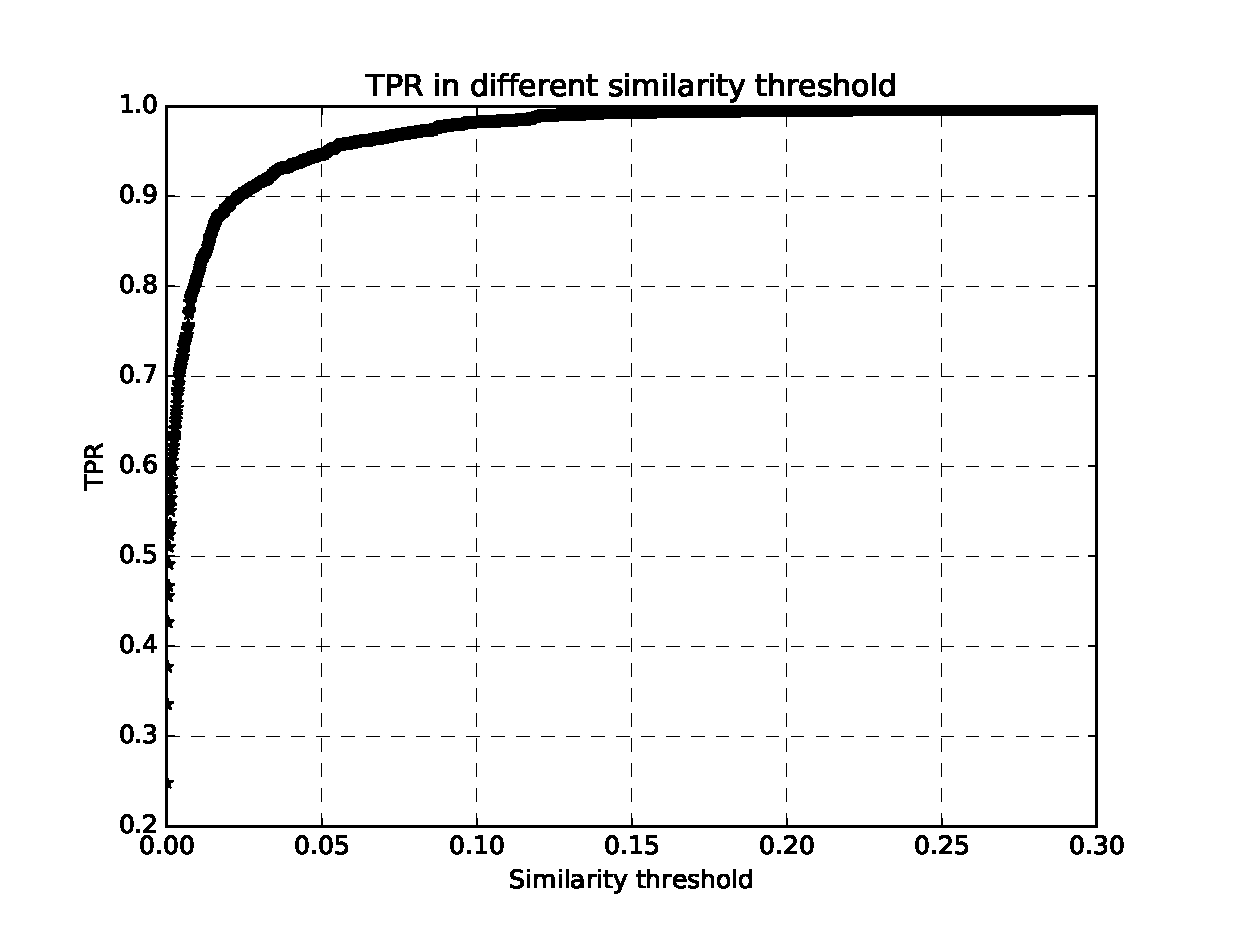
\includegraphics[width=0.30\textwidth]{threasholdcopy.eps}}
   \hspace{0.1in}
   \subfigure[]{\label{2} 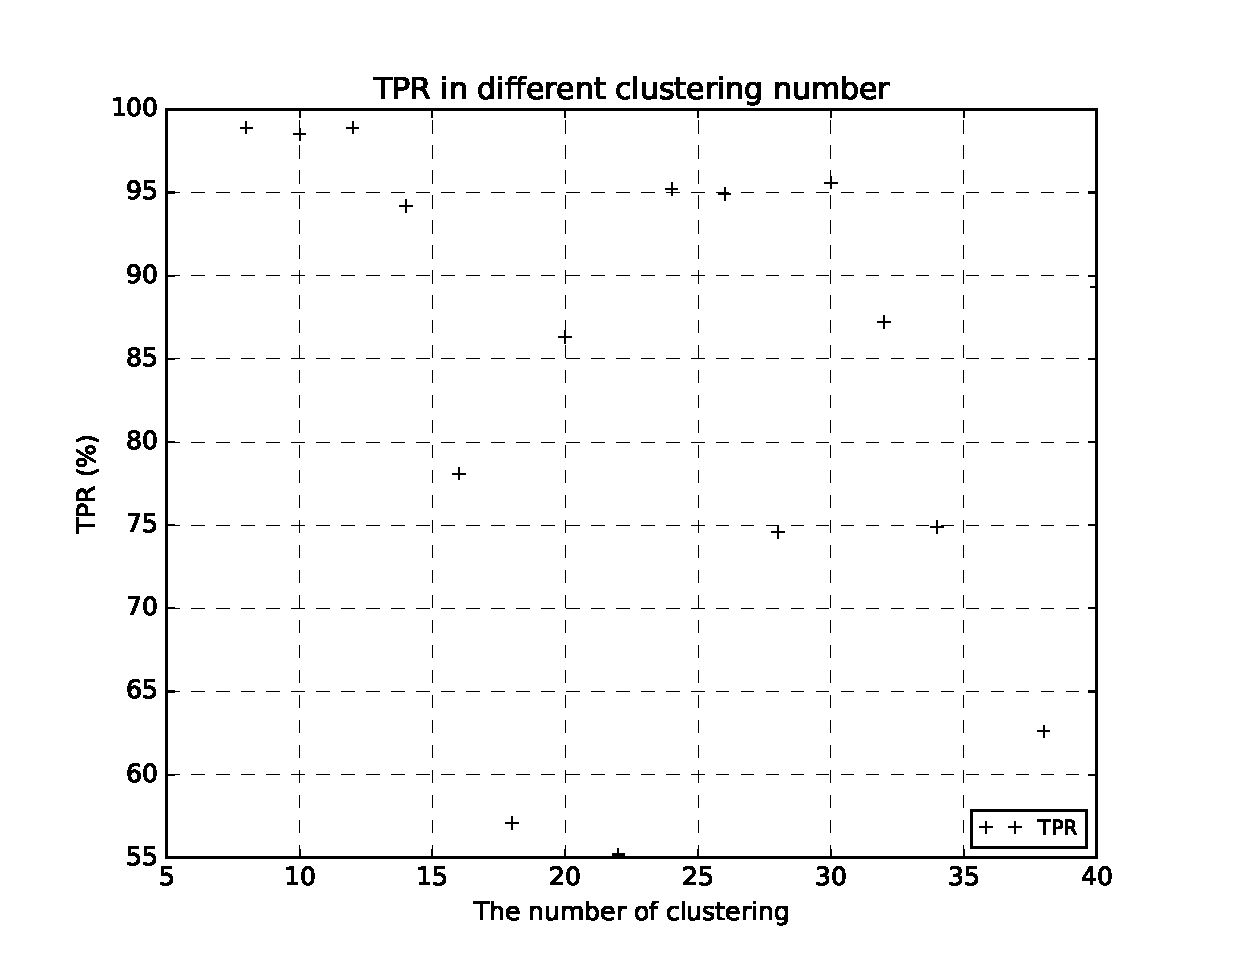
\includegraphics[width=0.30\textwidth]{clustercopy.eps}} \hspace{0.1in}
   \subfigure[]{\label{3} 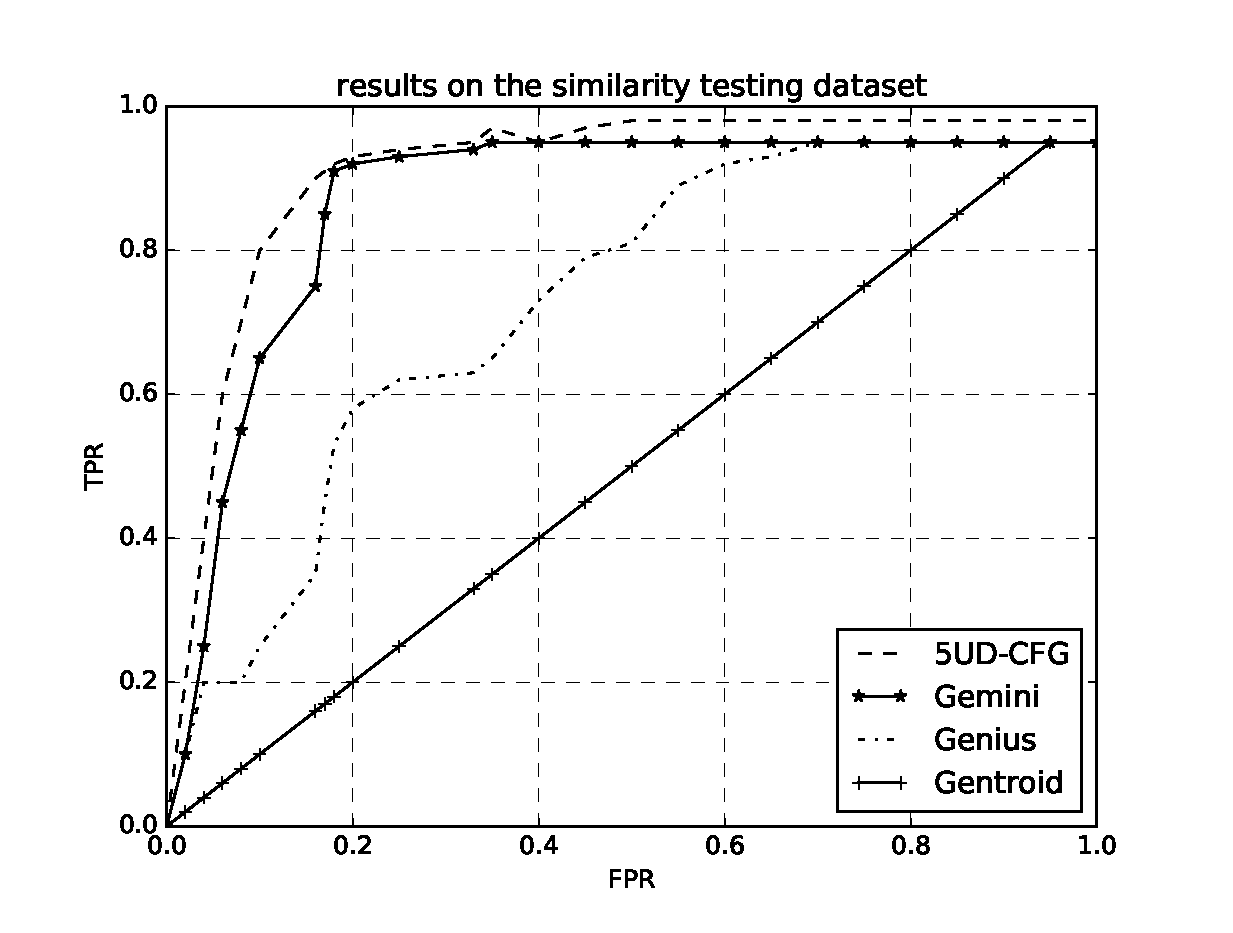
\includegraphics[width=0.30\textwidth]{TPRcopy.eps}}\\
   \caption{Accuracy}
   \vspace{-3 mm}
   \end{figure*}

%\begin{figure}[hbt]
%  \center{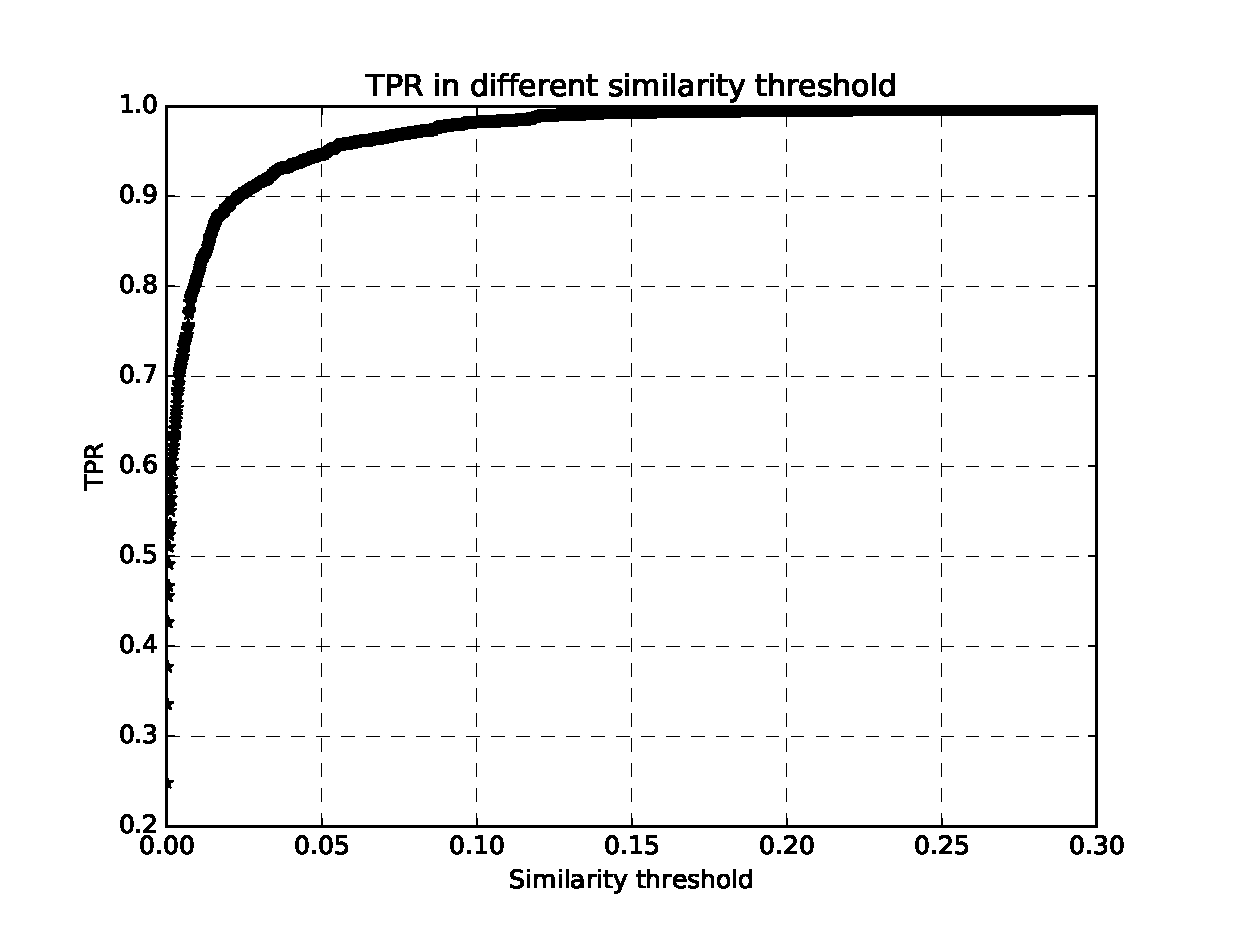
\includegraphics[width=8cm] {threasholdcopy.eps}}
%  \caption{\label{1}  TPR with different threashold}
%\end{figure}

Based on the proposed clustering algorithm in Algorithm 1, the different clustering's number affects TPR. Fig. 4 (b) shows that there is a inflection point in the changing curve of relationship between the clustering number and the TPR. We can see that TPR is the largest if the clustering number is $0.014\%$ of the number of search database. 
%\begin{figure}[hbt]
%  \center{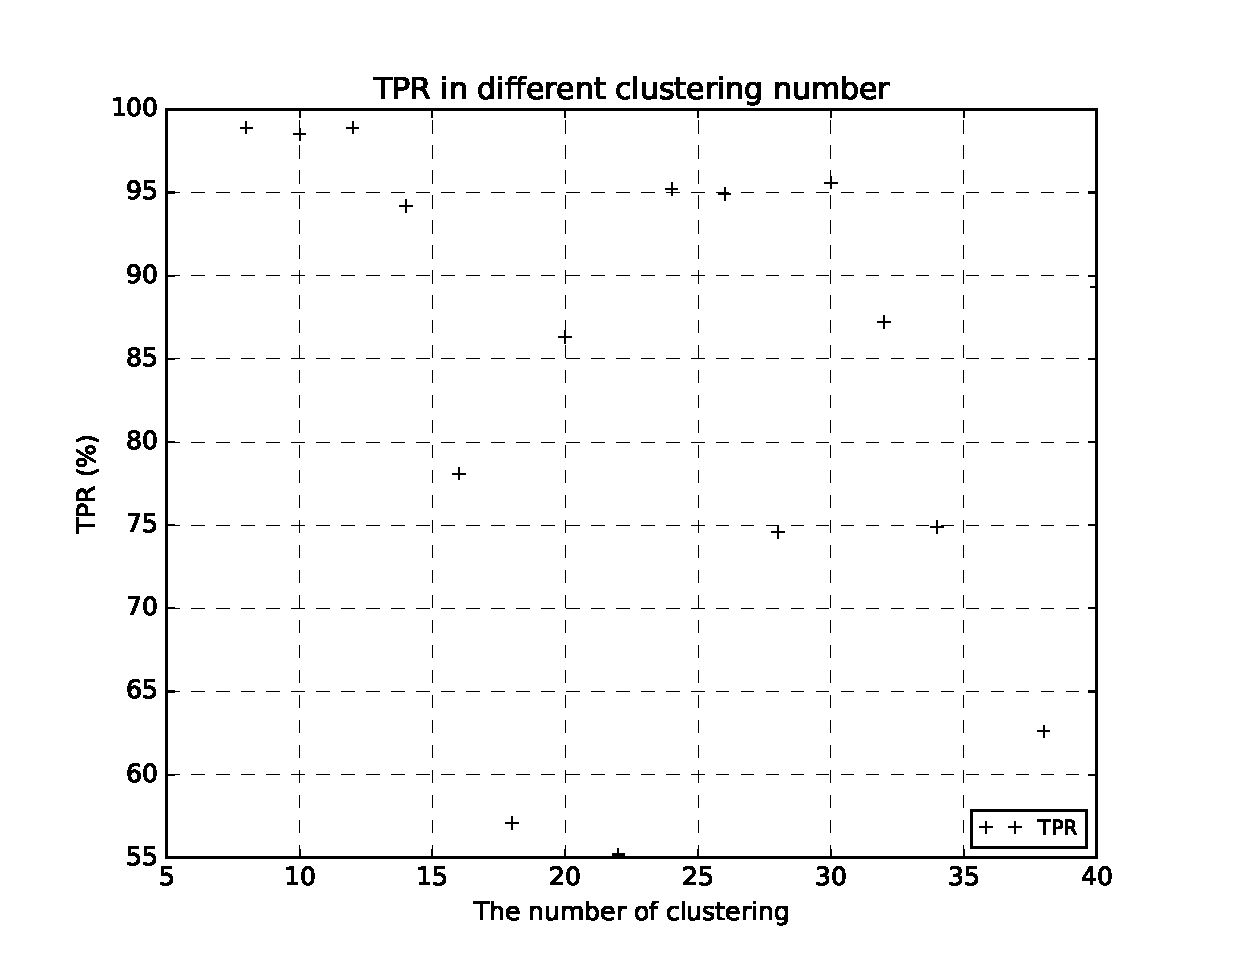
\includegraphics[width=8cm] {clustercopy.eps}}
%  \caption{\label{2}  TPR with different clustering number}
%\end{figure}

To compare the efficacy of final 3TU-CFG with centroid, gemini and genius, we use the same testing data to calculate the ROC curve in the same threshold. We use two metrics to evaluate the accuracy of the proposed and compared methods:the true positive rate (TPR) and the false positive rate (FPR). %For the searched samples query $q$, there are $m$ matching functions out of total of $L$ functions. If we set the first $F$ results as the positives, the total number of the correct matched functions $c$, which are true positive. The remaining number of functions in the $F$ functions, that is $F-c$, are false positives. We set the TPR as $TPR=\frac{c}{m}$ and the false positive rate is $FPR=\frac{F-c}{L-m}$. 

%\begin{figure}[hbt]
%  \center{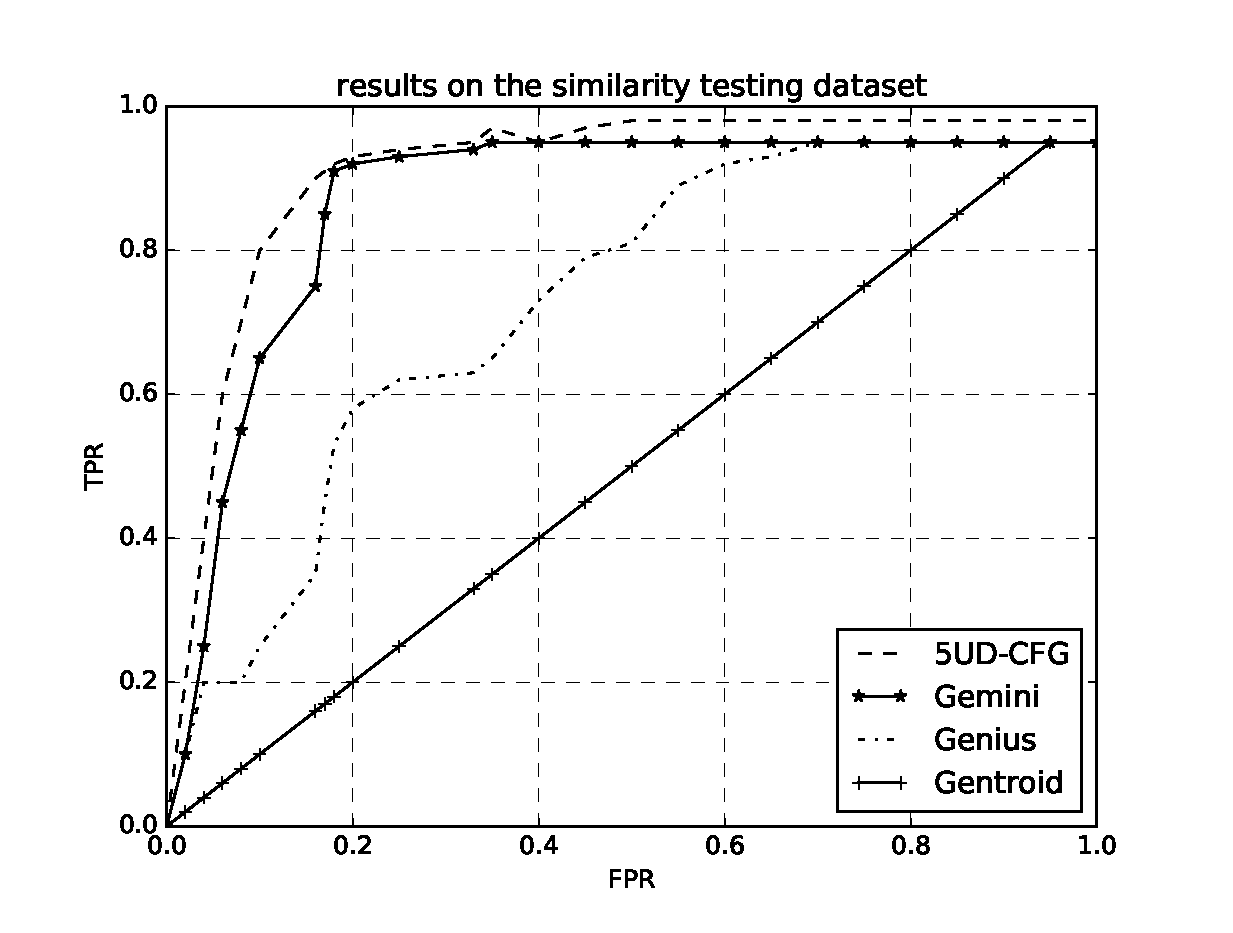
\includegraphics[width=8cm] {TPRcopy.eps}}
%  \caption{\label{3}  ROC on the similarity testing dataset}
%\end{figure}


%描述图7,比较三个方法。后面就是时间的实验部分。
We use $2082$ apps in the testing database as the queries to match with the target approaches. Fig. 4 (c) shows evaluating results of the ROC curve. we can see that 3TU-CFG outperforms another three approaches: Gemini, Genius, and Centroid. The size of ROC curve of 3TU-CFG is the largest, which shows the 3TU-CFG is the most accurate. When the FPR is small, TPR is significantly better than other approaches. Four curves show that TPR is increasing with FPR increasing. However, the rate of ROC curve of 3TU-CFG has the fastest growing. The results shows the 3TU-CFG can achieve even better accuracy than other approaches.

We consider search results and observe the advanced performance of 3TU-CFG is mainly because the 5UD-CFG can monotonously represent a function (proved in Section 4) and 3TU-CFG is obtained by monotonously compressing 5UD-CFG. Each function just need a closest candidate to make sure the accuracy for 3TU-CFG embedding process. The Gemini need train several iterations to get the embedding vector of the function. The model that is trained by the neural network needs a mount of samples to make sure the accuracy. Genius has several candidates that the accuracy depends on the accuracy of the codebook. Centroid has a great gap between different platforms, which is not monotonously represent the function. Our method is adept in representing entire structure of CFG, distinguishing the change, and thus shows the better results. 

According to our tensor model, we know that each benign function in a benign app have a benign label that denoted as $1$. If there is a malware function in a app, we consider this app is a suspicious app. For the suspicious apps found by our model, we validated them through online virus detection system and manual evaluations to judge the validity of our detection. 

%\subsubsection{Accuracy in the App Detection}
 
\subsection{Efficiency Comparison}
We measure the scalability of proposed approach from the following three aspects: the scale of the five collective markets, the performance on app homology detection and update of the basic feature database.

We analyze all apps in the collective five markets to obtain a basic database. Fig. 5 shows the distribution of size per app and the number for this app, the distribution of opcodes per app and the number for this kind of opcodes, and the distribution of the number of methods per app and the number for this app. We train in total $152, 789$ apps are in these five groups. Fig. 5 (a) shows that the size of nearly $94.7\%$  apps is in $0-50 MB$. The total size of apps is $7.47~TB$. The Fig. 5 (b) shows that nearly $69.8\%$ apps have $1-16000$ methods, and nearly $77.6\%$ apps have more than $4000$ methods.  

\begin{figure*}[hbt]
   \centering
   \subfigure[]{\label{1} 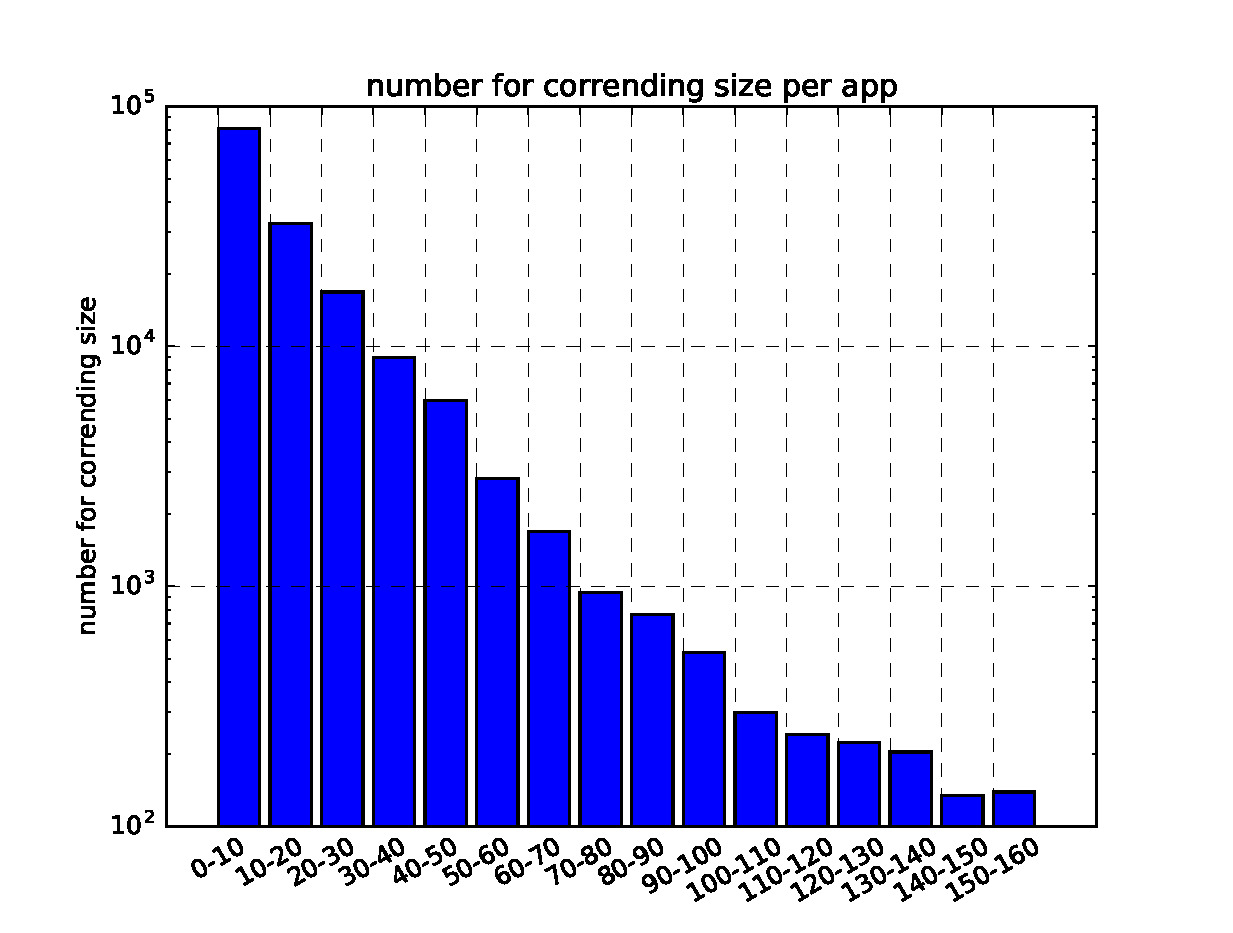
\includegraphics[width=0.30\textwidth]{numbercopy.eps}}
   \hspace{0.1in}
   \subfigure[]{\label{2} 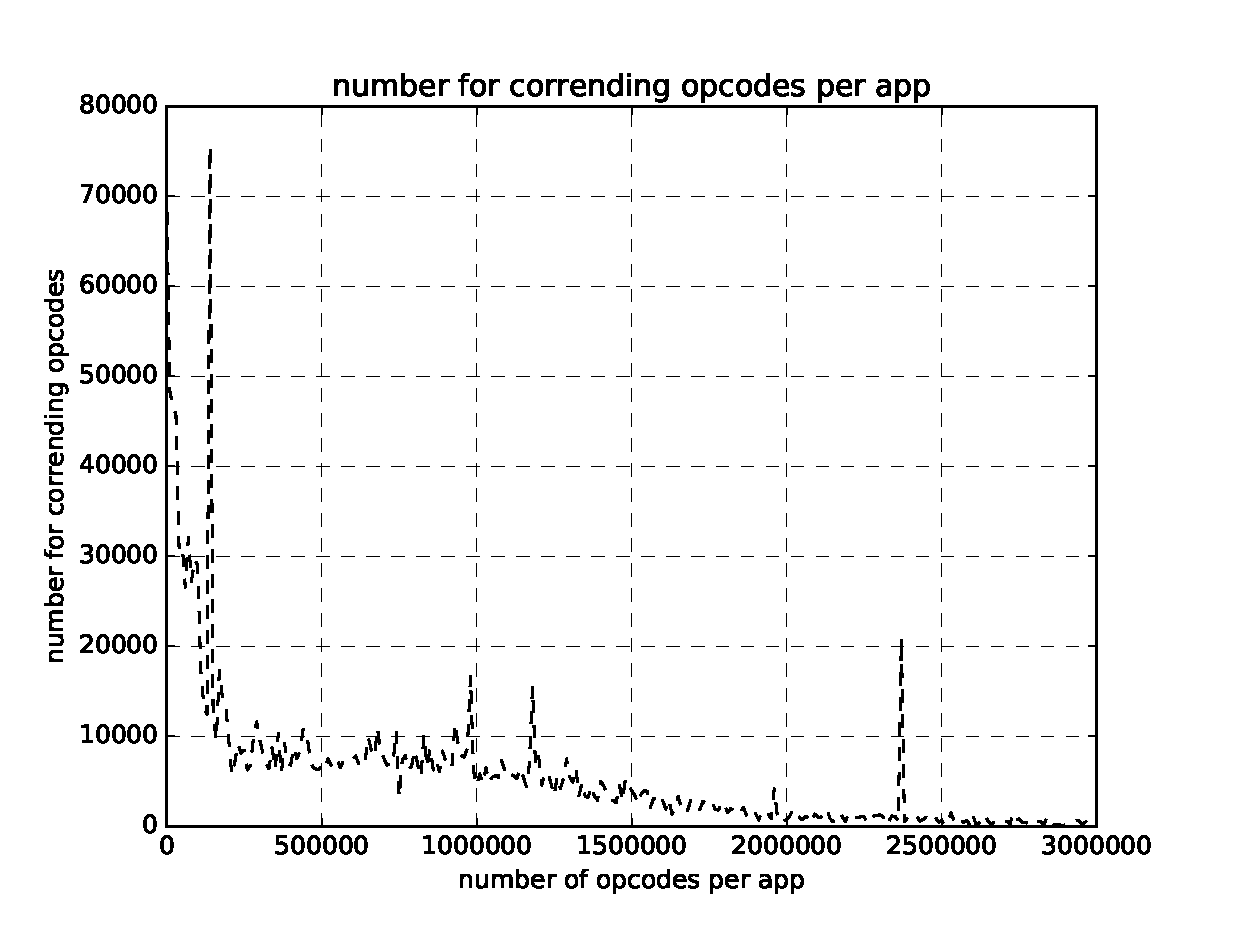
\includegraphics[width=0.30\textwidth]{opcodecopy.eps}} \hspace{0.1in}
   \subfigure[]{\label{3} 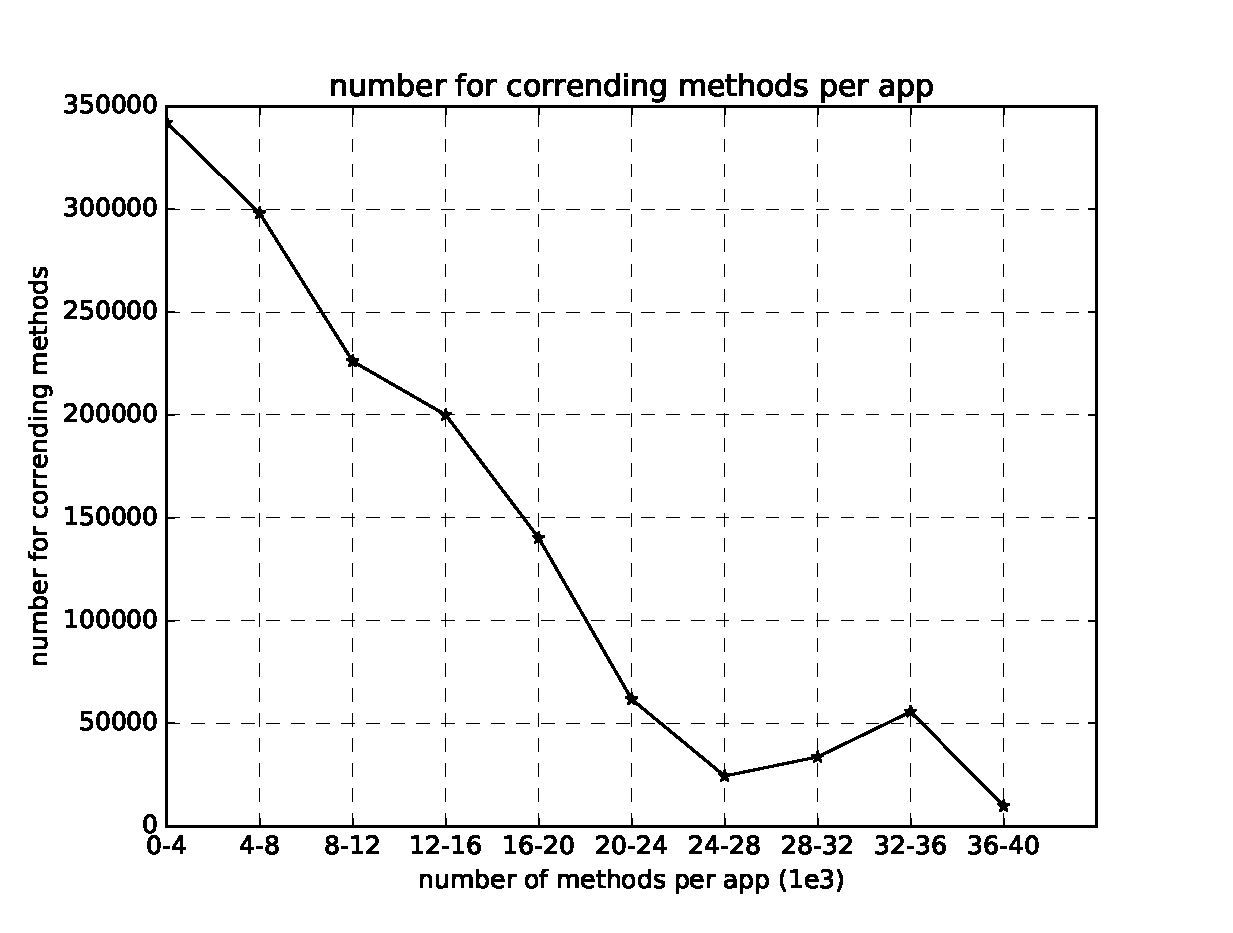
\includegraphics[width=0.30\textwidth]{methodcopy.eps}}\\
   \caption{Scalability of the database.}
   \vspace{-3 mm}
   \end{figure*}

We investigate the time consumption for each stage to demonstrate that 3TU-CFG is capable of handling apps at a large scale: 1) CFG with attributes extraction time, 2) embedding generation time, 3) Update time, and 4)app homology search time.

The time of the embedding generation depends on the total size of apps. We need to decompile the app into a series of functions. This step can be done in parallel. We use the androguard to obtain the original CFG structure. The original CFG generation time is the decompile time of the app. We can use several computer to measure the time. At the same time, Fig. 6 compare the 3TU-CFG embedding generation time with other three approaches, which including the decompile time. We store the CFG embedding vector in the database, and then use the KNN to search and detection. Then we evaluate the efficiency of Gemini, Genius for embedding time and Centroid for centroid generation time. 

\begin{figure*}[hbt]
   \centering
   \subfigure[]{\label{1} 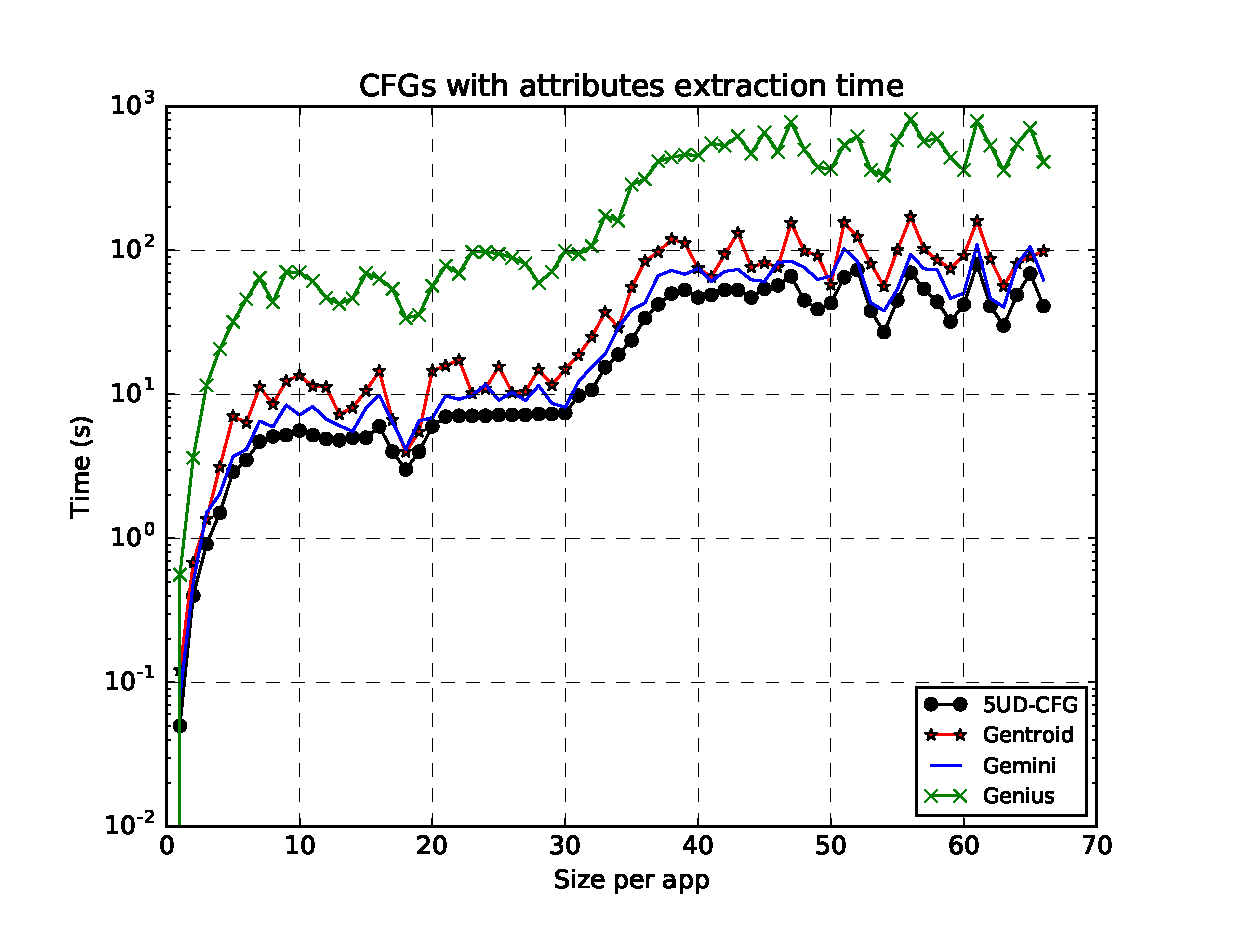
\includegraphics[width=0.30\textwidth]{extracttimecopy.eps}}
   \hspace{0.1in}
   \subfigure[]{\label{2} 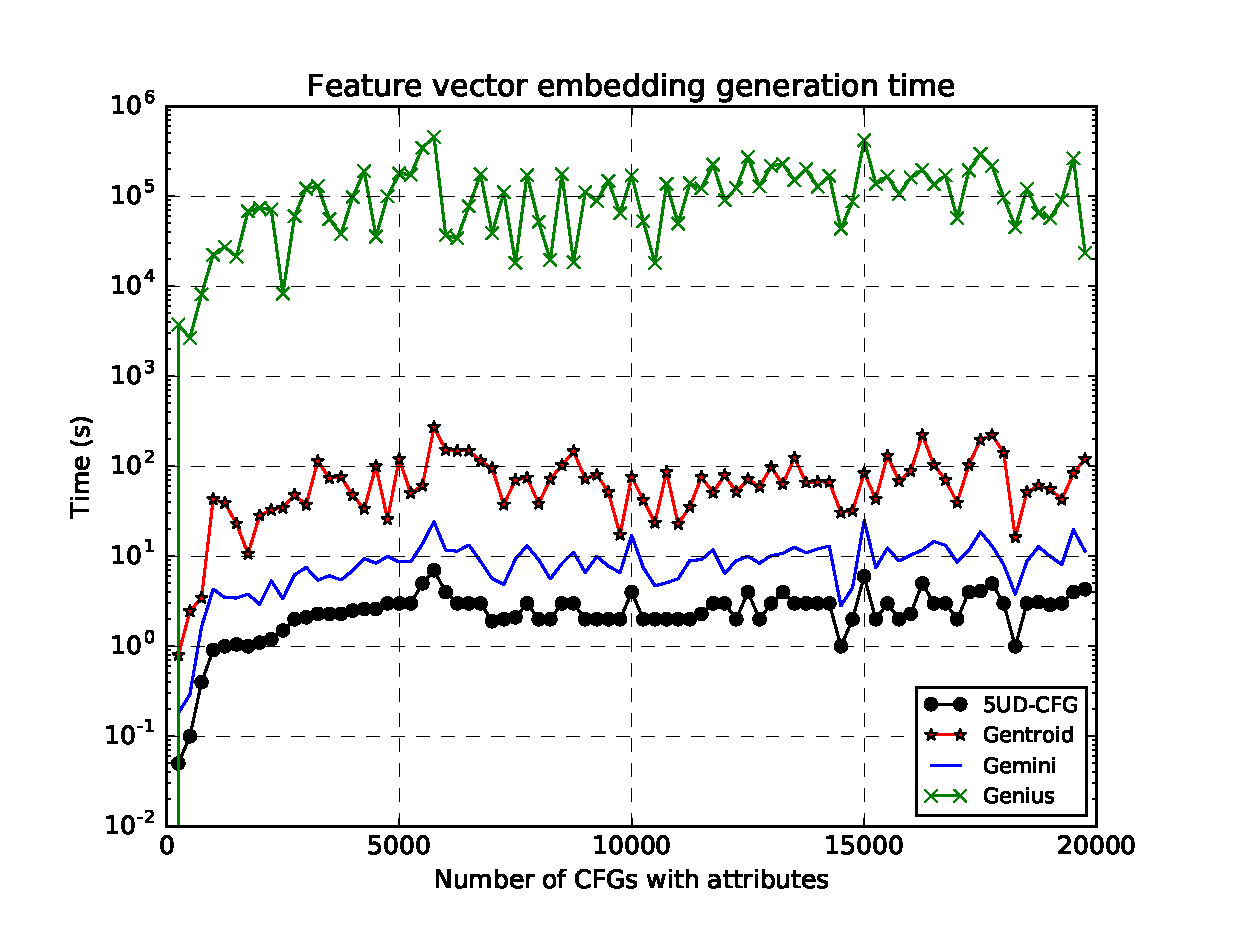
\includegraphics[width=0.30\textwidth]{embeddingtimecopy.eps}} \hspace{0.1in}
   \subfigure[]{\label{3} 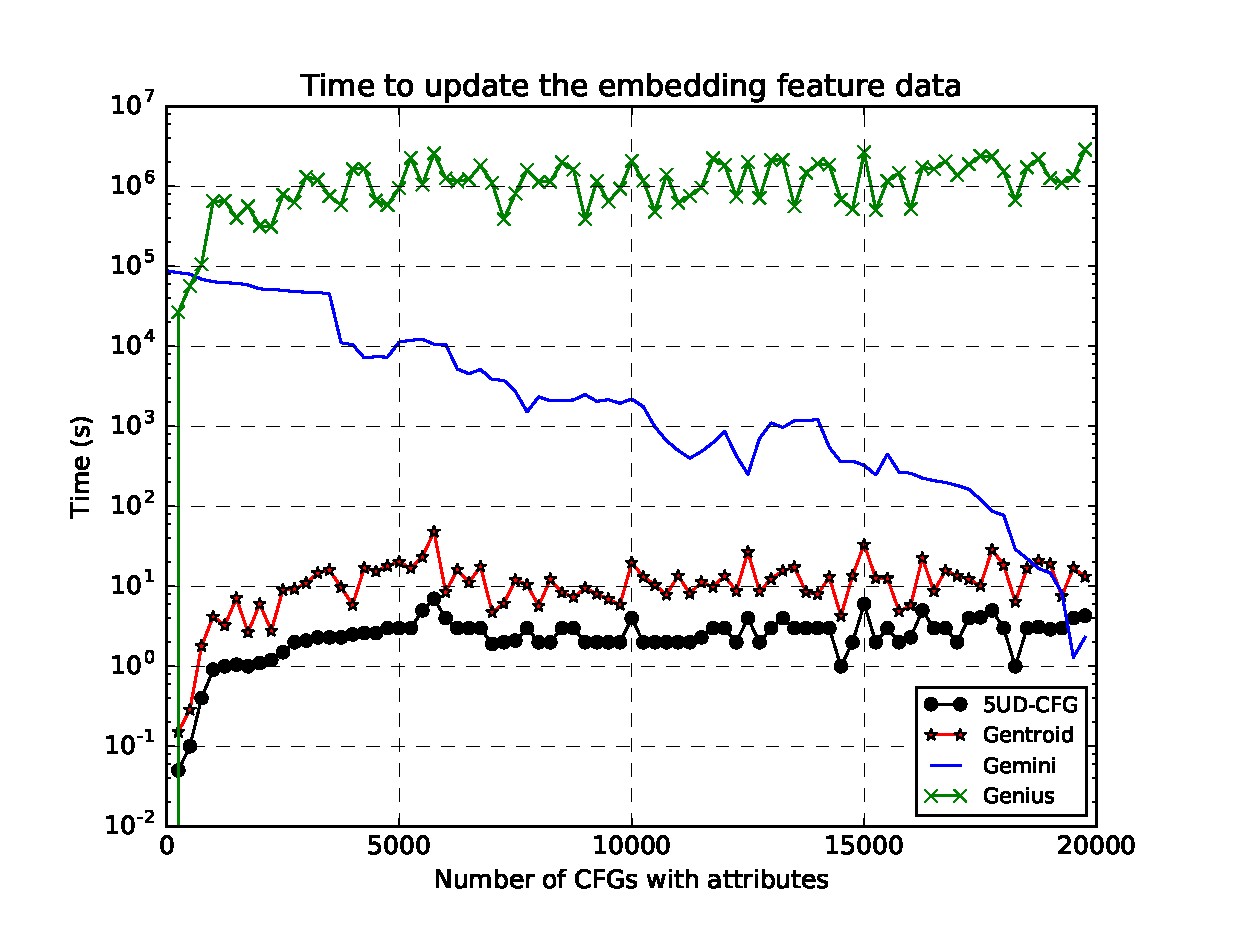
\includegraphics[width=0.30\textwidth]{updatetimecopy.eps}}\\
   \caption{Efficiency evaluation.}
   \vspace{-3 mm}
   \end{figure*}
 
 \begin{figure*}[!hbt]
   \centering
   \subfigure[]{\label{1} \includegraphics[width=0.30\textwidth]{searchtime_final.eps}}
   \hspace{0.1in}
   \subfigure[]{\label{2} \includegraphics[width=0.30\textwidth]{geniussearchtime_final.eps}} \hspace{0.1in}
   \subfigure[]{\label{3} \includegraphics[width=0.30\textwidth]{centroidseartime_final.eps}}\\
   \caption{Search time in scalable feature data.}
   \vspace{-3 mm}
   \end{figure*}


\subsubsection{Performance on CFG with attributes extraction time.}

Fig. 6 (a) shows the CFG with attributes extraction times of 5UD-CFG can improve upon Genius by $8\times$ to $15\times$ on average on CFG embedding time. The 5UD-CFG needs to extract 5 basic-block attributes along with the structure feature of the CFG. However, Genius needs to additionally extract the betweenness attributes, in total 8 attributes. The different becomes larger for the app with a large size. A app with the large size has more methods. There are more nodes in a CFG. It needs more time to compute the betweenness attributes for larger size's app with a amount of nodes. The preparation times of the 5UD-CFG can improve upon Gemini by $1.1\times$ to $1.7\times$ on average for different sizes of apps. Gemini needs to extract 6 basic-block attributes and the number of offspring time. However, Gemini aggregate the graph structural information through iterations of embedding update. Therefore, the CFG with attributes extraction times of the 3TU-CFG is close to Gemini. Centroid also extract 5 basic-block attributes with the structure feature, the process is similar to the CFG with attributes extraction process of the 5UD-CFG. The CFG with attributes extraction times of the 5UD-CFG is close to Centroid. 

\subsubsection{Performance on embedding generation time.}

Fig. 6 (b) shows the embedding generation time for four approaches with the increasing number of methods. The number of method denotes the scalable of the CFG. Obviously, more methods need more embedding time. 3TU-CFG, Genius, Gemini and Centroid all transform the CFG of the function to the embedding vector. We can see 3TU-CFG run $4700\times$ to $76000\times$ faster than Genius, run $2.1\times$ to $5\times$ faster than Gemini, and run $7\times$ to $51\times$ faster than Centroid on average. Since 3TU-CFG embedding process avoids the complexed neural network learning process, the expensive graph matching and the scalable clustering algorithm. Genius needs extra time to generate the codebook for all CFGs by the complex bipartite graph matching. Gemini needs extra time to learn five iterations for obtaining the CFG embedding feature. Centroid is to compute the centroid of a spatial geometry. This preparation process is simpler than the above two approaches. Therefore, the preparation time of Centroid is lower than another two approaches. However, the embedding process of the 3TU-CFG is more concise than other three approaches. The line embedding and the tensor embedding have much simpler matrix operations than that in the neural network iteration computation. However, Gemini and 3TU-CFG belong to the matrix operation, which can be parallelized.      


\subsubsection{Performance on Update time.}

Fig. 6 (c) shows the update feature database time. Adding new apps is very common in android markets. If the new app is not included in the database, we need to update the database. We can see that the update time of 3TU-CFG is quicker $4\times$ to $20000\times$ than Gemini, quicker more than $180000\times$ than Genius, and quicker $2\times$ to $7\times$ than Centroid. If we just update few apps at once, the different of time between the 3TU-CFG and the Gemini is larger. Since we propose a incremental algorithm of tenor embedding that just needs to retrain the increasing novel methods rather than retrain all feature vector. If the number of novel methods are same with the number of original feature data. The update embedding time of 3TU-CFG is close to Gemini. Since the Gemini need to embed all ACFGs to get the update feature data although it does not need to regenerate ACFGs. Specifically, Genius needs to retrain the codebook, this is a larger project, which means regenerate all feature vector including scalable graph matching algorithm. It costs too much time. Centroid just needs to update the increasing apps. However, it's accuracy is lower than the 3TU-CFG. Therefore, 3TU-CFG has a better performance on the update.
%We evaluate the scalability of 3TU-CFG on the collective five app markets, which consist of in total $152, 789$ apps. We investigate the time consumption for each stage to demonstrate that 3TU-CFG is capable of handling apps at a large scale. 

\subsubsection{App homology search time.} 
Fig. 7 (a) shows the search time for 3TU-CFG in the larger scale codebase. We choose five collective dataset into six codebases of different scales from $c=10^3$ to $c=10^8$, where $c$ is the total number of functions in the codebase. We choose the $1$ to $10000$ sequentially submitted queries. As we can see, the search time grows like linearly according to the increase of the codebase size, and the average search time is close to $4.6 \times 10^{(-9)}$. Fig. 7 (b) shows the search time for Gemini and Genius, these two approaches use the same propose LSH search method and the number of the feature vector are also same. Therefore, they have the same distribution of the search time. We can see the search time of the 3TU-CFG run $2\times$ faster than Genius and Gemini on average. Since the 3TU-CFG finally has a 3-eigenvalues vector, half as many as the feature vector of Genius and Gemini. The search method use the KNN search algorithm. Fig. 7 (c) shows the search time for Centroid, 3TU-CFG run $10\times$ to $100\times$. Since Centroid use the binary search for a 5-eigenvalues vectors, which is slower than KNN with a 3-eigenvalues vector. Therefore, 3TU-CFG has the less search time for scalable database.




%There have been several existing works for the function clone and other works for app clone:   


\section{Related Work}

We discuss the closest related works in this Section. We focus on approaches using code similarity to search for known malware apps. There are many other approaches that aim at finding unknown malware.

\textbf{Binary-level function clone detection.} One common approaches is that trace-based approach \cite{DavidY14} captures execution sequences as features for code similarity checking, which can detect the CFG changes. However, this approach does not accurately find the malware codes across different architectures. Static birthmarks \cite{KhooMA13}\cite{AndrewsVSS17} are usually the characteristics in the code that cannot easily be modified such as constant values in field variables, a sequence of method calls, an inheritance structure and used classes. Rendezvous \cite{KhooMA13} first explored the code search in binary code. However, it has two limitations. It relies on ngram features to improve the search accuracy. Secondly, it decomposes the whole CFG of a function into subgraphs. Jannik \cite{FengZXCTY16} \cite{LiuCZLXCS17} propose a system to derive bug signatures for known bugs. They compute semantic hashes for the basic blocks of the binary. When can then use these semantics to find code parts in the binary that behave similarly to the bug signature, effectively revealing code parts that contain the bug. However, it can not be scalable. Deqiang Fu et al. \cite{DFuXYY17} proposed a control flow graph-based malware detection method. They extract features named ``code chunks" from the control flow graph, then use the classification and regression tree (CART) algorithm to classify these features. The method can obtain $96.3\%$ classification accuracy.

\textbf{App clone detection.} Most existing approaches identify malicious apps \cite{EnckGCCJMS14} \cite{JustEM15} typically rely on heavyweight static or dynamic analysis techniques, and cannot detect the unknown malware whose behavior has not been modeled a priori. PiggyApp\cite{ZhouZGJZ13} \cite{0012WLWZHZ015} \cite{DuWL17} \cite{ArpSHGR14} utilize the features (permissions, API, etc.) identified from a major component shared between two apps to find other apps also including this component, then clusters the rest part of these apps' code and samples from individual clusters to manually determine whether the payloads are indeed malicious. In dynamic app cone analysis, applications are executed in a virtual environment. Runtime information is recorded to generate dynamic features for malware detection. For example,  ANDRUBIS \cite{ArpSHGR14}\cite{unknown} dynamically examined the operations for over 1 million apps in four years, which is an off-line analyzer for recovering detailed behavior of individual malicious apps. Enck et al. \cite{DEnckGHTCCJMS14} \cite{EgeleWCB14} \cite{YanY12} proposed TaintDroid, a virtualization-based malware detection method that can trace the flow of sensitive information. In an evaluation of 30 Android applications, TaintDroid found 20 applications had misused users’ private information. However, it has a worse limitation that can not be scalable to handle millions and thousands of apps.

%Yao \cite{DuWL17} present a new malware detection method that automatically divides a function call graph into community structures. The features of these community structures can then be used to detect malware. Arp et al. \cite{ArpSHGR14} proposed a lightweight detection method called DREBIN. This method can extract eight types of static features from Android applications. These features are then input to vector space models for classification by a support vector machine (SVM) algorithm. Their method achieved $94\%$ detection accuracy on $123,453 $ Android applications.

%\textbf{Dynamic app clone detection}
%Another effective approach for malware detection that is resistant to code confusion mechanisms is dynamic analysis. In dynamic app cone analysis, applications are executed in a virtual environment. Runtime information is recorded to generate dynamic features for malware detection. For example,  ANDRUBIS \cite{ArpSHGR14}\cite{unknown} dynamically examined the operations for over 1 million apps in four years, which is an off-line analyzer for recovering detailed behavior of individual malicious apps. Enck et al. \cite{DEnckGHTCCJMS14} proposed TaintDroid, a virtualization-based malware detection method that can trace the flow of sensitive information. In an evaluation of 30 Android applications, TaintDroid found 20 applications had misused users’ private information. However, it has a worse limitation that can not be scalable to handle millions and thousands of apps. Blanket-execution \cite{EgeleWCB14} uses the dynamic run-time environment of the program as features to conduct the code search. This approach can defeat the CFG changes, but it is only evaluated in a single architecture. DroidScope \cite{YanY12} is also a virtualization-based malicious code detection method. It can identify malware by analyzing semantics features of operating system level and Java level. 






\section{Conclusion}
In this paper, we present a two-hierarchies embedding model to generate a feature vector for extracting CFG of app's functions. We propose a prototype called 3TU-CFG, which has a scalable and effective power on the app homology analysis. The embedding feature vector is carefully designed objective functions that preserve both the first-order and second-order proximities of CFG for functions, which is called 5UD-CFG. At the same time, we can prove the monotonous of first-hierarchy embedding 5UD-CFG. An effective and efficient compress and clustering algorithm based on the second-hierarchy tensor embedding model is proposed for generating 3TU-CFG. Our extensive evaluation shows that 3TU-CFG outperforms the current other approaches by large margins with respect to similarity detection accuracy, embedding generation time and overall search time. The real dataset demonstrate that 3TU-CFG significantly improve detection accuracy and search effective.      


\section*{Acknowledgment}
The paper is supported by China NSF (61572222, 61272405,61272033, 61272451,61472121) and China University Innovation Foundation (2013TS102, 2013TS106).

%\bibliographystyle{IEEEtran}
%\bibliography{MW.bib}
{\footnotesize \bibliographystyle{acm}
\bibliography{MW}}

%\theendnotes

\end{document}



